\chapter{Emulation of detector responses on MC simulation}
\label{ref:mc-emulation}

To ensure that the statistical uncertainties due to the limited size of the  MC
samples are small compared to those of data,
it is important to have MC samples with a size at least 4 times as large as
data.
Due to the sheer size of LHCb run 2 data
(a factor of $\sim\!1.26$ for 2016 alone compared to full run 1 despite smaller
integrated luminosity due to a larger \bbbar cross section and higher triggering
efficiencies),
it is not computationally possible to generate
enough full simulation (FullSim) MC, where every detector response is simulated.

It is estimated in Ref.~\cite{LHCb-INT-2019-025}
that about 85\% of the computation time is spent on simulating RICH and the
calorimeter system.
Tracker-only (TO) MC sets all but the tracking system of the detector to
passive material, making the simulation about 8 times faster than FullSim.
Hence, to reach the target statistical uncertainties,
TO MC is (almost) exclusively used for this analysis.
Therefore, detector responses like trigger and particle identification (PID)
need to be emulated offline.
The emulation procedures for these responses are described in the rest of the
chapter.


\section{Trigger emulation}
\subsection{Emulation of L0Hadron TOS}

As discussed in \cref{ref:sel:data},
the L0 trigger requirements for this analysis are:
either the \Dz candidate fires the L0 hadron trigger line
(\Dz L0Hadron TOS)
or the rest of the event aside from the \Dz\muon candidate (and its decay chain)
triggers at least one L0 trigger (\B L0Global TIS).
Note that ``TOS'' stands for \emph{Triggered On Signal} where
\emph{signal} in this case is the \Dz candidate,
and ``TIS'' means \emph{Trigger Independent of Signal} where the \emph{signal}
refers to the \Dz\muon pair.
For more information about trigger TIS, TOS, TISTOS, and TOB,
consult \cref{appx:trigger-cat}.

The L0 hadron line (L0Hadron) is triggered when the sum of the transverse
energy\footnote{
    Defined as: $E_T \equiv \sqrt{m^2 + p^2} \sin\theta$.
    In massless limit, $E_T = p_T$.
} $E_T$ deposited
in a single $2 \times 2$ HCAL cluster is above a set threshold\footnote{
    See Table 1 in \cite{LHCb-DP-2019-001} for year-by-year thresholds of each
    L0 trigger.
},
as described in Ref.~\cite{LHCb-DP-2019-001}.
For L0Hadron TOS, it is required that for all HCAL clusters associated with the
signal track (\Dz in this case),
with the association predicted by the tracking system,
the highest $E_T$ is above the triggering threshold.

Tracker-only MC records the tracker-predicted position where a track hits the
calorimeters.
Hence, though the triggering variable $E_T$ is not accessible,
variables related to $E_T$, or, equivalently, to the trigger decision, are.
It is conceivable that L0Hadron TOS can be emulated by providing
the relevant variables and the trigger decision to train a regressor,
which can in turn be used to predict trigger decisions based on the training
variables alone, without requiring emulating $E_T$ at all.
The emulation procedure, inspired by Ref.~\cite{LHCb-INT-2019-025}, is
described below:

\begin{enumerate}
    % \item The \smalltt{TupleToolL0Calo} tool is configured to save HCAL
    %     information.
    \item The training variables, listed in \cref{tab:l0-hadron-emu-vars}, and
        the trigger decision from a FullSim MC of decay
        $\Bz \rightarrow \Dstarp \mu \nu$, a normalization mode,
        are used to train \xgboost, a BDT-based regressor
        \cite{Chen:2016:XST:2939672.2939785}.
    \item Once the model is trained, with just the training variables,
        \xgboost predicts the probabilities of events passing L0 hadron trigger.
    \item The probabilities are applied as weights to a separate validation
        sample of the same FullSim MC to check the quality of the emulation.
        It is shown in \cref{fig:l0hadron-tos-emu} that the emulated L0Hadron
        TOS trigger has excellent agreement with the \emph{simulated} trigger in
        FullSim.
\end{enumerate}

\begin{table}[!htb]
    \caption{Variables used to train \xgboost for L0 hadron emulation.}
    \label{tab:l0-hadron-emu-vars}
    \centering
    \begin{tabular}{c|c}
        \toprule
        \bf Group   & \bf Variables \\
        \midrule
        Event-level & nTracks \\
        \Dz         & $p$, $p_T$ \\
        \midrule
        \Km         & \makecell{
                      $p$, $p_T$,
                      real $E_T$\parnote{
                          This is the $E_T$ measured by the tracker.
                          In massless limit, $E_T = p_T$.
                      }, \\
                      HCAL $x$-projection, HCAL $y$-projection,
                      HCAL region\parnote{
                          This indicates whether the hits are in the inner or
                          outer region of HCAL.
                          The outer region has a coarser granularity than the
                          inner, thus it is more likely that the energies from
                          \Km and \pip are deposited in the same cluster,
                          enhancing L0Hadron TOS efficiency.
                      }} \\
        \midrule
        \pip        & same as \Km \\
        \bottomrule
    \end{tabular}
    \begin{flushleft}
        \parnotes
    \end{flushleft}
\end{table}

% Generated in //lhcb-ntuples-gen/studies/trigger_emulation-l0_hadron_tos_debug:
% By running:
%   git annex get .
%   debug_l0hadron.py
% in the folder specified above.
\begin{figure}
    \centering
    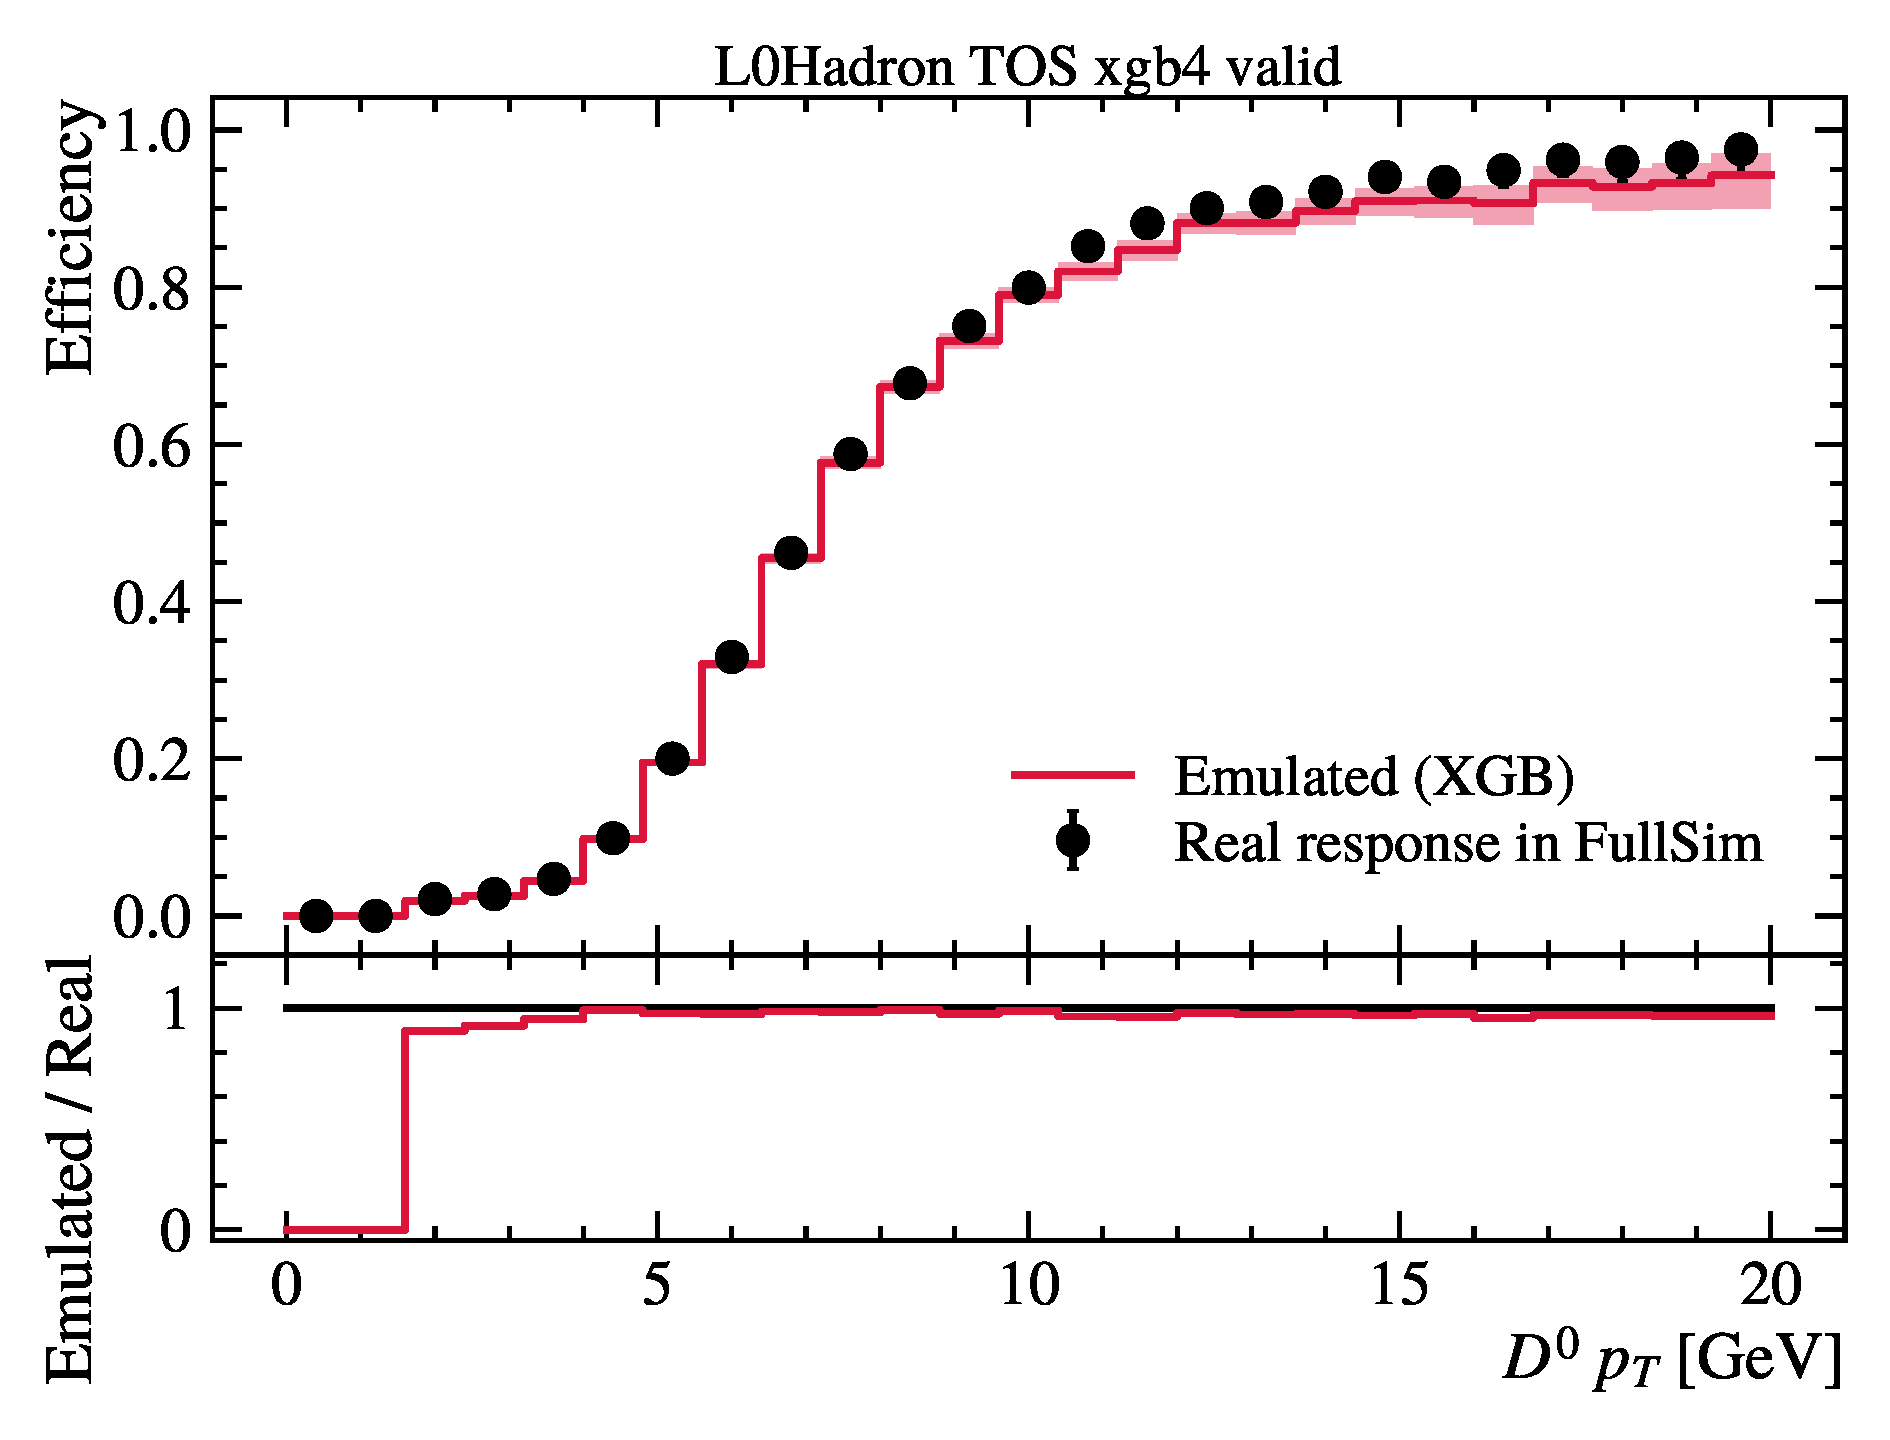
\includegraphics[width=0.7\textwidth]{./figs-mc-emulation/emulate-l0hadron-tos/b0_L0Hadron_TOS_xgb4_valid_d0_pt.pdf}
    \caption{
        The emulated trigger probabilities applied as a weight to FullSim has
        excellent agreement with real L0Hadron TOS trigger \emph{simulated} in
        FullSim.
    }
    \label{fig:l0hadron-tos-emu}
\end{figure}


\subsection{Emulation of L0Global TIS}

As discussed before, L0Global TIS is determined by \emph{the rest of event}
(everything but the reconstructed \B decay chain) which is \emph{not saved}
after event reconstruction.
Therefore, a completely different approach is needed for its emulation.

Instead of predicting the event-by-event L0Global TIS probability based on the
properties of the rest of event,
it is possible to measure the L0Global TIS efficiencies binned in
\emph{certain reconstructed variables\footnote{
    The choice of variables will be discussed later.
}},
and then apply L0Global TIS efficiencies based on the bin the event falls
in.

In addition, for hadron colliders,
the rest of event is \emph{busy} due to hadronization:
Indeed, for data reconstructed in the
$\Bm \rightarrow \Dz (\rightarrow \Km \pip) \mun \neumb$ mode which is used in
this analysis,
the average number of tracks per event is 170,
whereas the selected \Dz\mun final state contains only 3 tracks (\Km, \pip, and
\mun, as \Dz and \Bm are reconstructed from these tracks)!
Therefore, it can be argued that the rest of event is essentially the same
for different $B$ decays,
and L0Global TIS efficiencies are portable.
%
Assuming the L0Global TIS efficiencies can be measured in a data
sample reconstructed in a particular decay mode, the measured efficiencies
can be applied to TO MC as weights regardless of the simulated decays.

To summarize, if the following assumptions hold, then the emulation outlined
above should work:

\begin{enumerate}
    \item The L0Global TIS efficiencies can be measured in data.
    \item The L0Global TIS efficiencies do not depend on \B decay mode.
\end{enumerate}

Before we proceed, let us define L0Global TIS efficiency
$\epsilon_\text{L0Global TIS}$ more precisely.
According to \cite{LHCb-PUB-2014-039}, in LHCb $\epsilon_\text{L0Global TIS}$
is conventionally defined as:

\begin{equation}
    \label{eqn:eff-l0global-tis}
    \epsilon_\text{L0Global TIS} \equiv
    \frac{N_\text{L0Global TIS \& selected}}{N_\text{selected}}
\end{equation}
which is not directly evaluable in real data, as $N_\text{selected}$ refers to
the number of selected events \emph{regardless} of their trigger decisions.
% which is not measurable (in data).

However, the conditional efficiency, $\epsilon_\text{L0Global TIS|L0Muon TOS}$,
is measurable:

\begin{equation}
    \epsilon_\text{L0Global TIS|L0Muon TOS} \equiv
    \frac{N_\text{L0Global TIS \& L0Muon TOS \& selected}}{
          N_\text{L0Muon TOS \& selected}}
\end{equation}
as long as L0Muon TOS and all L0 triggers (L0Global) on the rest of event are
uncorrelated,
$\epsilon_\text{L0Global TIS|L0Muon TOS}$ is equivalent to
$\epsilon_\text{L0Global TIS}$.
Such a method is called \emph{TISTOS method}.
Unfortunately, there is a correlation between the two triggers due to
the fact that \bbbar are produced in pairs,
making the kinematics of the selected signal \B meson and the background \Bbar
meson,
part of rest of event, correlated.

Still, it is argued in Ref.~\cite{LHCb-PUB-2014-039}
that L0Global TIS and L0Muon TOS are \emph{uncorrelated} in a small region of
signal \B phase space.
In Ref.~\cite{LHCb-INT-2019-025} it is checked that binned
$\epsilon_\text{TISTOS} = \epsilon_\text{TIS}$ in
$\B \rightarrow \jpsi K$ FullSim MC\footnote{
    TISTOS does not always work. See \cref{appx:suppl:l0global-tis} for a
    counter example.
},
and evaluated that
$\epsilon_\text{L0Global TIS}$ on data reconstructed in $\jpsi K$,
binned in $\log(p_z)$ and $\log(p_T)$ of the \B meson.
It is also checked that the efficiencies are portable among
$\B \rightarrow \jpsi K$, $\B \rightarrow \Dp \muon \neu$, and
$\B \rightarrow \Dp \tauon \neu$ decays with MC samples.
Thus, it is possible to measure $\epsilon_\text{L0Global TIS}$ \emph{binned} in
\B kinematic variables with the TISTOS method.

In \cref{fig:l0global-tis-portable} we check
that the portability still holds for this analysis in
$\B \rightarrow \Dstarp \muon \neu$ and $\B \rightarrow \Dstarp \tauon \neu$.
The efficiencies obtained in Ref.~\cite{LHCb-INT-2019-025} are applied to all TO
MC samples in this analysis as a function of the true momenta,
as the reconstruction in this analysis contains missing neutrino(s),
whereas $\jpsi K$ does not.

% Generated in /lhcb-ntuples-gen/studies/trigger_emulation-l0_global_tis_debug:
% By running:
%   debug_l0global.py
% in the folder specified above.
\begin{figure}[ht]
    \centering
    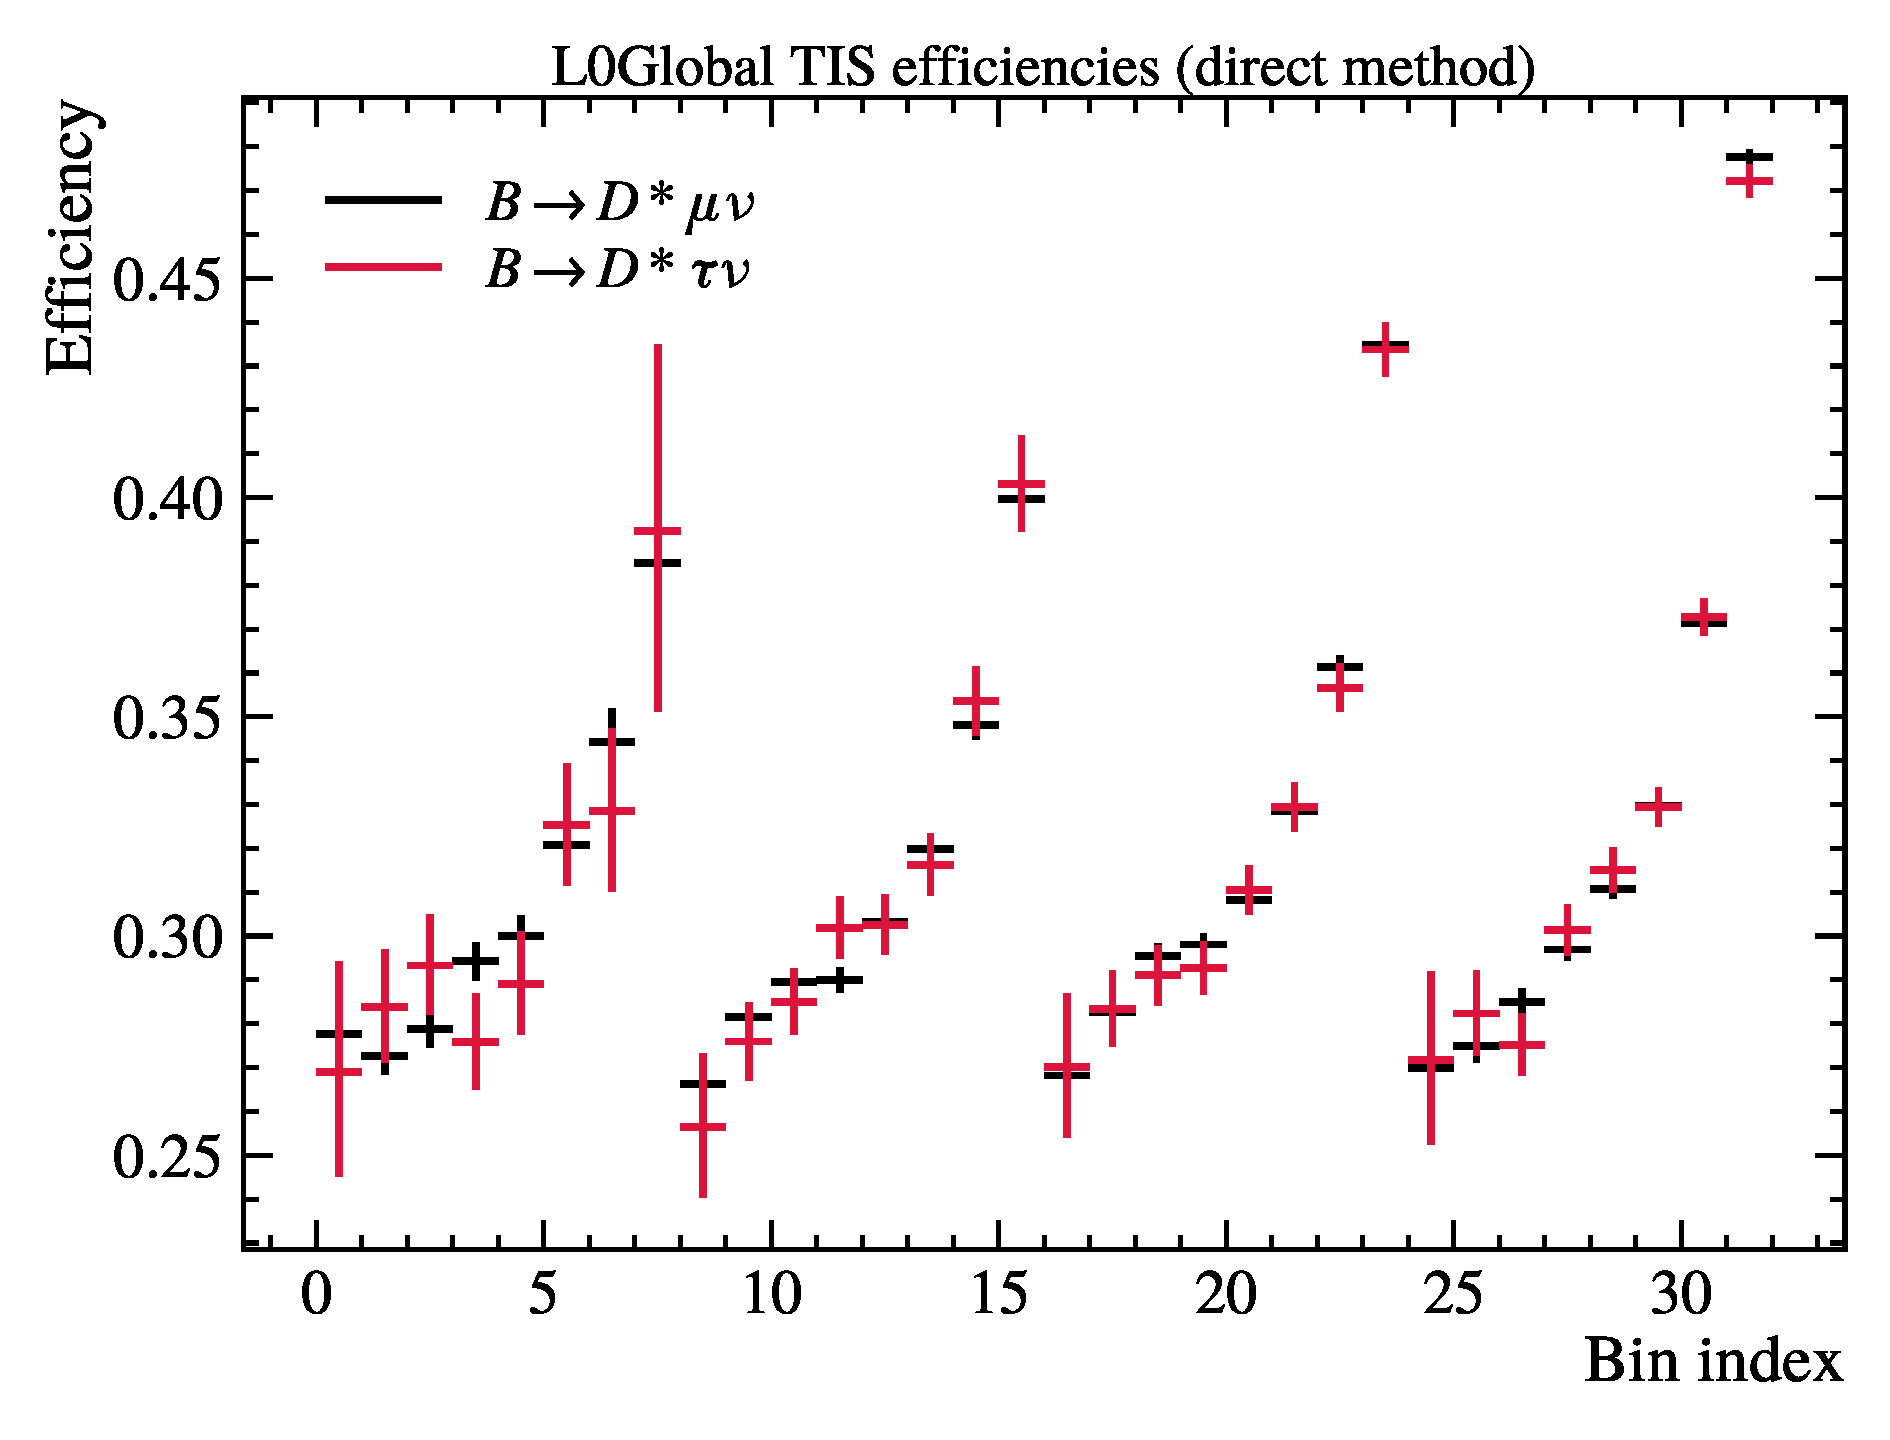
\includegraphics[width=0.32\textwidth]{
        ./figs-mc-emulation/emulate-l0global-tis/l0_global_tis_eff_bin_idx_dir.pdf
    }
    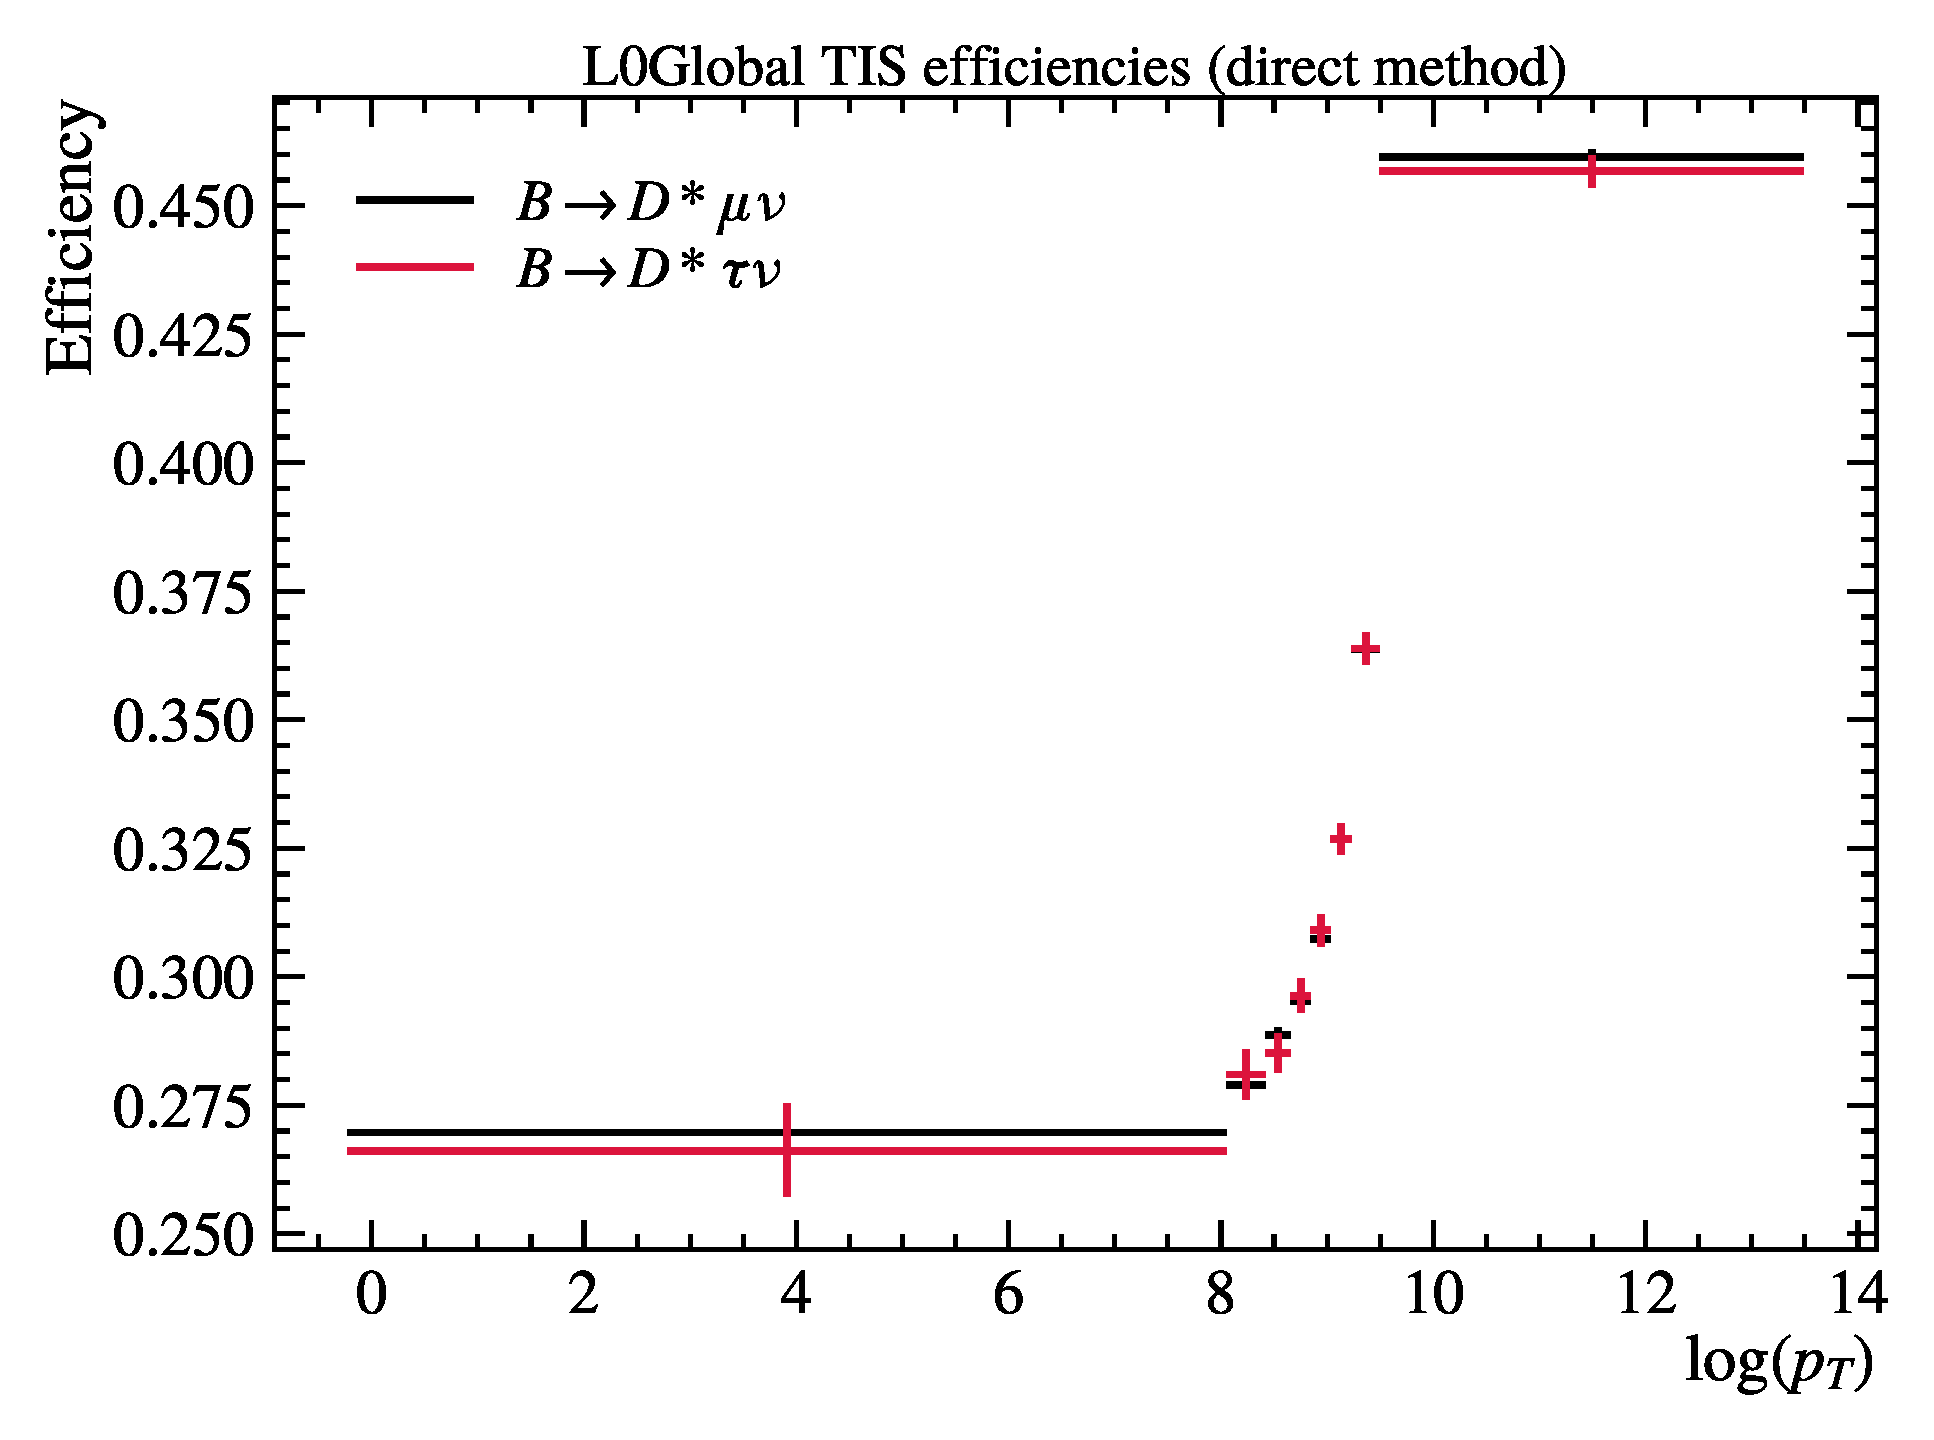
\includegraphics[width=0.32\textwidth]{
        ./figs-mc-emulation/emulate-l0global-tis/l0_global_tis_eff_log_pt_dir.pdf
    }
    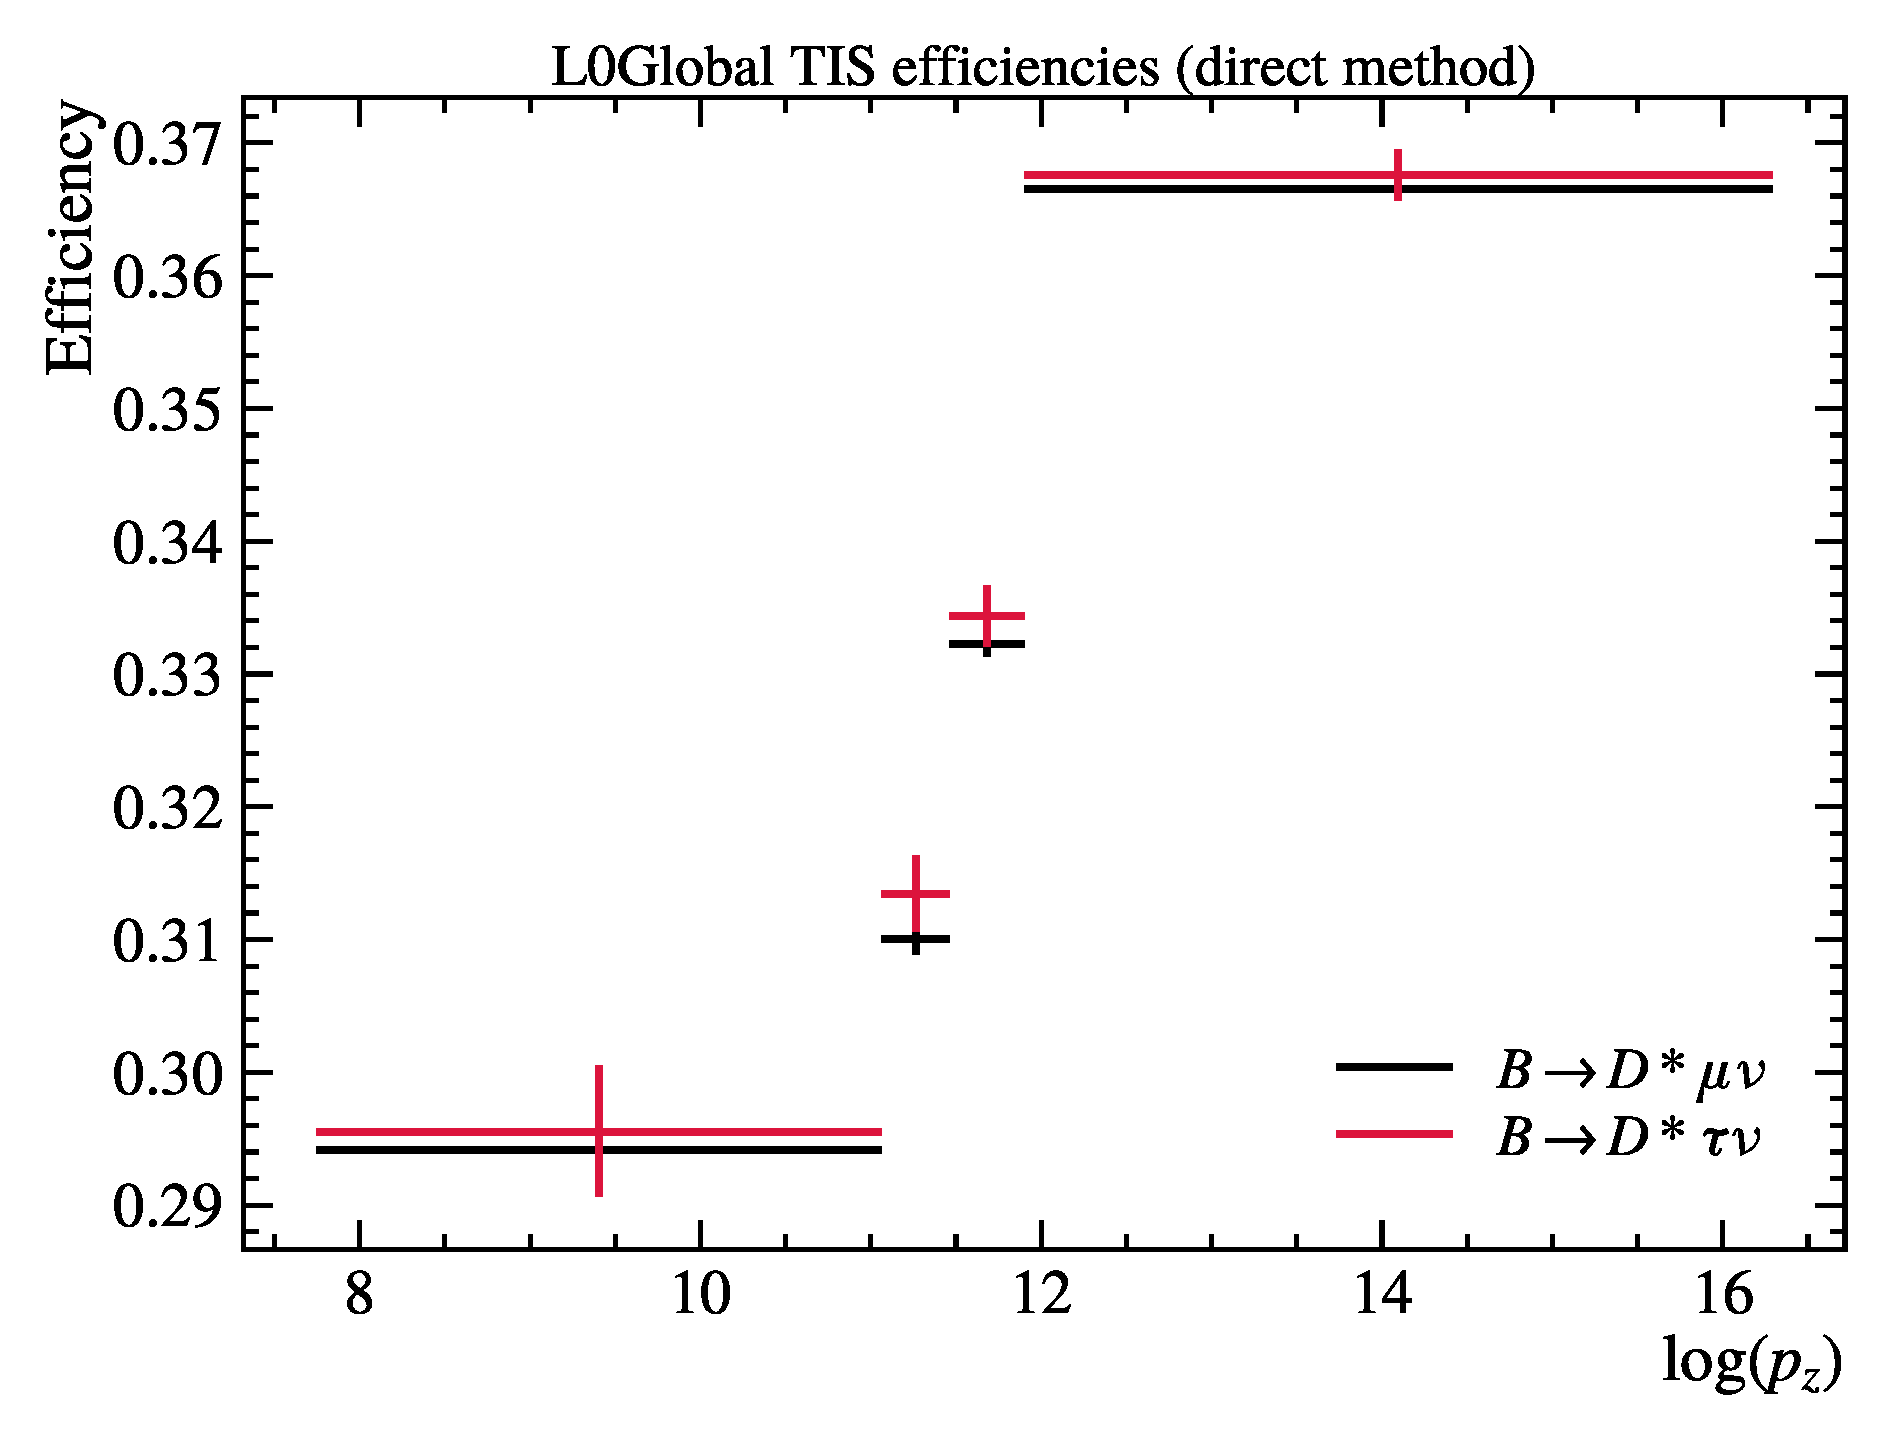
\includegraphics[width=0.32\textwidth]{
        ./figs-mc-emulation/emulate-l0global-tis/l0_global_tis_eff_log_pz_dir.pdf
    }
    \caption[Check that L0Global TIS is portable among signal and normalization MC modes]{
        Check that L0Global TIS is portable among signal and normalization MC modes

        The $p_T$ and $p_z$ momenta are MC true momenta of the $B$ meson.
        Bin index represents the index from an unrolled 2D
        true-$p_T$-true-$p_z$ histogram.
        Efficiencies are evaluated according to \cref{eqn:eff-l0global-tis},
        as the MC samples used here are \emph{not} filtered on trigger decision,
        so $N_\text{selected}$ can be evaluated directly.

        Efficiencies are in good agreement across all bins.
    }
    \label{fig:l0global-tis-portable}
\end{figure}


\subsection{Correlation between L0Hadron TOS and L0Global TIS}
\label{ref:mc-emulation:correlation-tos-tis}

L0 triggers have a global event cut on the number of SPD hits.
For all but the DiMuon trigger\footnote{
    Ignore Muon high \pt line for now.
}, the cut is placed at 450; for DiMuon, 900,
as listed in \cite{LHCb-INT-2019-025}.
For events that are both \emph{TIS and TOS}, a non-trivial correlation is
introduced by this cut, because it affects the L0 TIS efficiencies
inconsistently:
On a small patch of the signal \B phase space,
for events that are TIS on \emph{non-DiMuon}, TIS and TOS efficiency is:

\begin{equation}
    \epsilon_\text{TIS and TOS} =
        \epsilon_\text{L0-non-DiMuon TIS} \cdot \epsilon_\text{L0Hadron TOS}
\end{equation}

For L0DiMuon TIS only, however, its efficiency is affected by the SPD cut:
\begin{align}
    \epsilon_\text{L0DiMuon TIS \& nSPDhits < 450} & \neq
        \epsilon_\text{L0DiMuon TIS} \\
    \Rightarrow \epsilon_\text{TIS and TOS} & =
            \epsilon_\text{L0DiMuon TIS \& nSPDhits < 450} \cdot
            \epsilon_\text{L0Hadron TOS} \\
        & \neq
        \epsilon_\text{L0DiMuon TIS} \cdot \epsilon_\text{L0Hadron TOS}
\end{align}

Therefore:
\begin{align}
    \epsilon_\text{TIS and TOS} & =
        (\epsilon_\text{L0-non-DiMuon TIS} +
         \epsilon_\text{DiMuon TIS \& nSPDhits < 450}) \cdot
         \epsilon_\text{L0Hadron TOS} \\
    & \neq
        \underbrace{\epsilon_\text{L0Global TIS}}_{
            = \epsilon_\text{L0-non-DiMuon TIS} +
              \epsilon_\text{L0DiMuon TIS}
         } \cdot\; \epsilon_\text{L0Hadron TOS}
\end{align}

To minimize the correlation, a $\text{nSPDhits} < 450$ is applied on all data
samples\footnote{
    It is applied on the $\jpsi K$ sample as well, the one used to obtain
    binned L0Global TIS efficiencies.
    For TO MC, there is no nSPDhits variable.
}, which removes about an additional 4.4\% of candidates for both \Dz and
\Dstar channel.
After the SPD cut is applied, it is checked that
$\epsilon_\text{TIS or TOS} \approx \epsilon_\text{TIS} + \epsilon_\text{TOS} -
\epsilon_\text{TIS} \cdot \epsilon_\text{TOS}$
in \cite{LHCb-INT-2019-025},
that is, TIS efficiencies can be considered as uncorrelated from
TOS efficiencies.


\subsection{Emulation of \texttt{Hlt1TrackMVA} and \texttt{Hlt1TwoTrackMVA}}

The event selection requires that either $K$ or $\pi$ is TOS on
\smalltt{Hlt1TrackMVA},
or \Dz is TOS on \smalltt{Hlt1TwoTrackMVA}.
The single track \smalltt{Hlt1TrackMVA} requires a track that has a score based
on $p_T$ and \ipChiSq to be above some threshold;
the two track \smalltt{Hlt1TwoTrackMVA} feeds the $p_T$ and \ipChiSq of both
tracks to a \smalltt{MatrixNet} MVA,
requiring the two-track combination to pass the MVA selection.

All required variables are present in TO MC, and are extracted by adding
a tool\footnote{
    Named \lstinline{RelInfoHLT1Emulation}, available at
    \url{https://github.com/umd-lhcb/TrackerOnlyEmu/tree/master/davinci/Phys},
    courtesy of the authors of \cite{LHCb-INT-2019-025}.
} to event reconstruction.
%
The HLT1 triggers also require events to pass Global Event Cuts (GEC),
as listed in \cref{tab:gec},
to remove high-pile-up events.
There is also an online-offline difference:
The real HLT1 triggers use VELO-TT tracks which require at least three hits
in the TT,
whereas the emulation can only use VELO tracks which have no TT requirement.
Therefore, additional cuts and a 4.2\% penalty factor are imposed to account for
the differences.
The HLT1 trigger cuts and GEC are listed in \cite{LHCb-INT-2019-025}.
The emulated HLT1 are in good agreement with the real response in FullSim, as
can be seen in \cref{fig:hlt1-trackmva-emu,fig:hlt1-twotrackmva-emu}.

\begin{table}[!htb]
    \centering
    \caption{Global event cuts for HLT1. Taken from \cite{LHCb-INT-2019-025}.}
    \label{tab:gec}
    \begin{tabular}{c}
        \toprule
        {\bf Global event cuts (GEC)} \\
        \midrule
        50 < \texttt{nVeloClusters} < 6000 \\
        50 < \texttt{nITClusters} < 3000 \\
        50 < \texttt{nOTClusters} < 15000 \\
        \bottomrule
    \end{tabular}
\end{table}


% Generated in /lhcb-ntuples-gen/studies/plot-trigger_emulation, run the script:
%   trigger_emulation.sh
\begin{figure}[!htb]
    \centering
    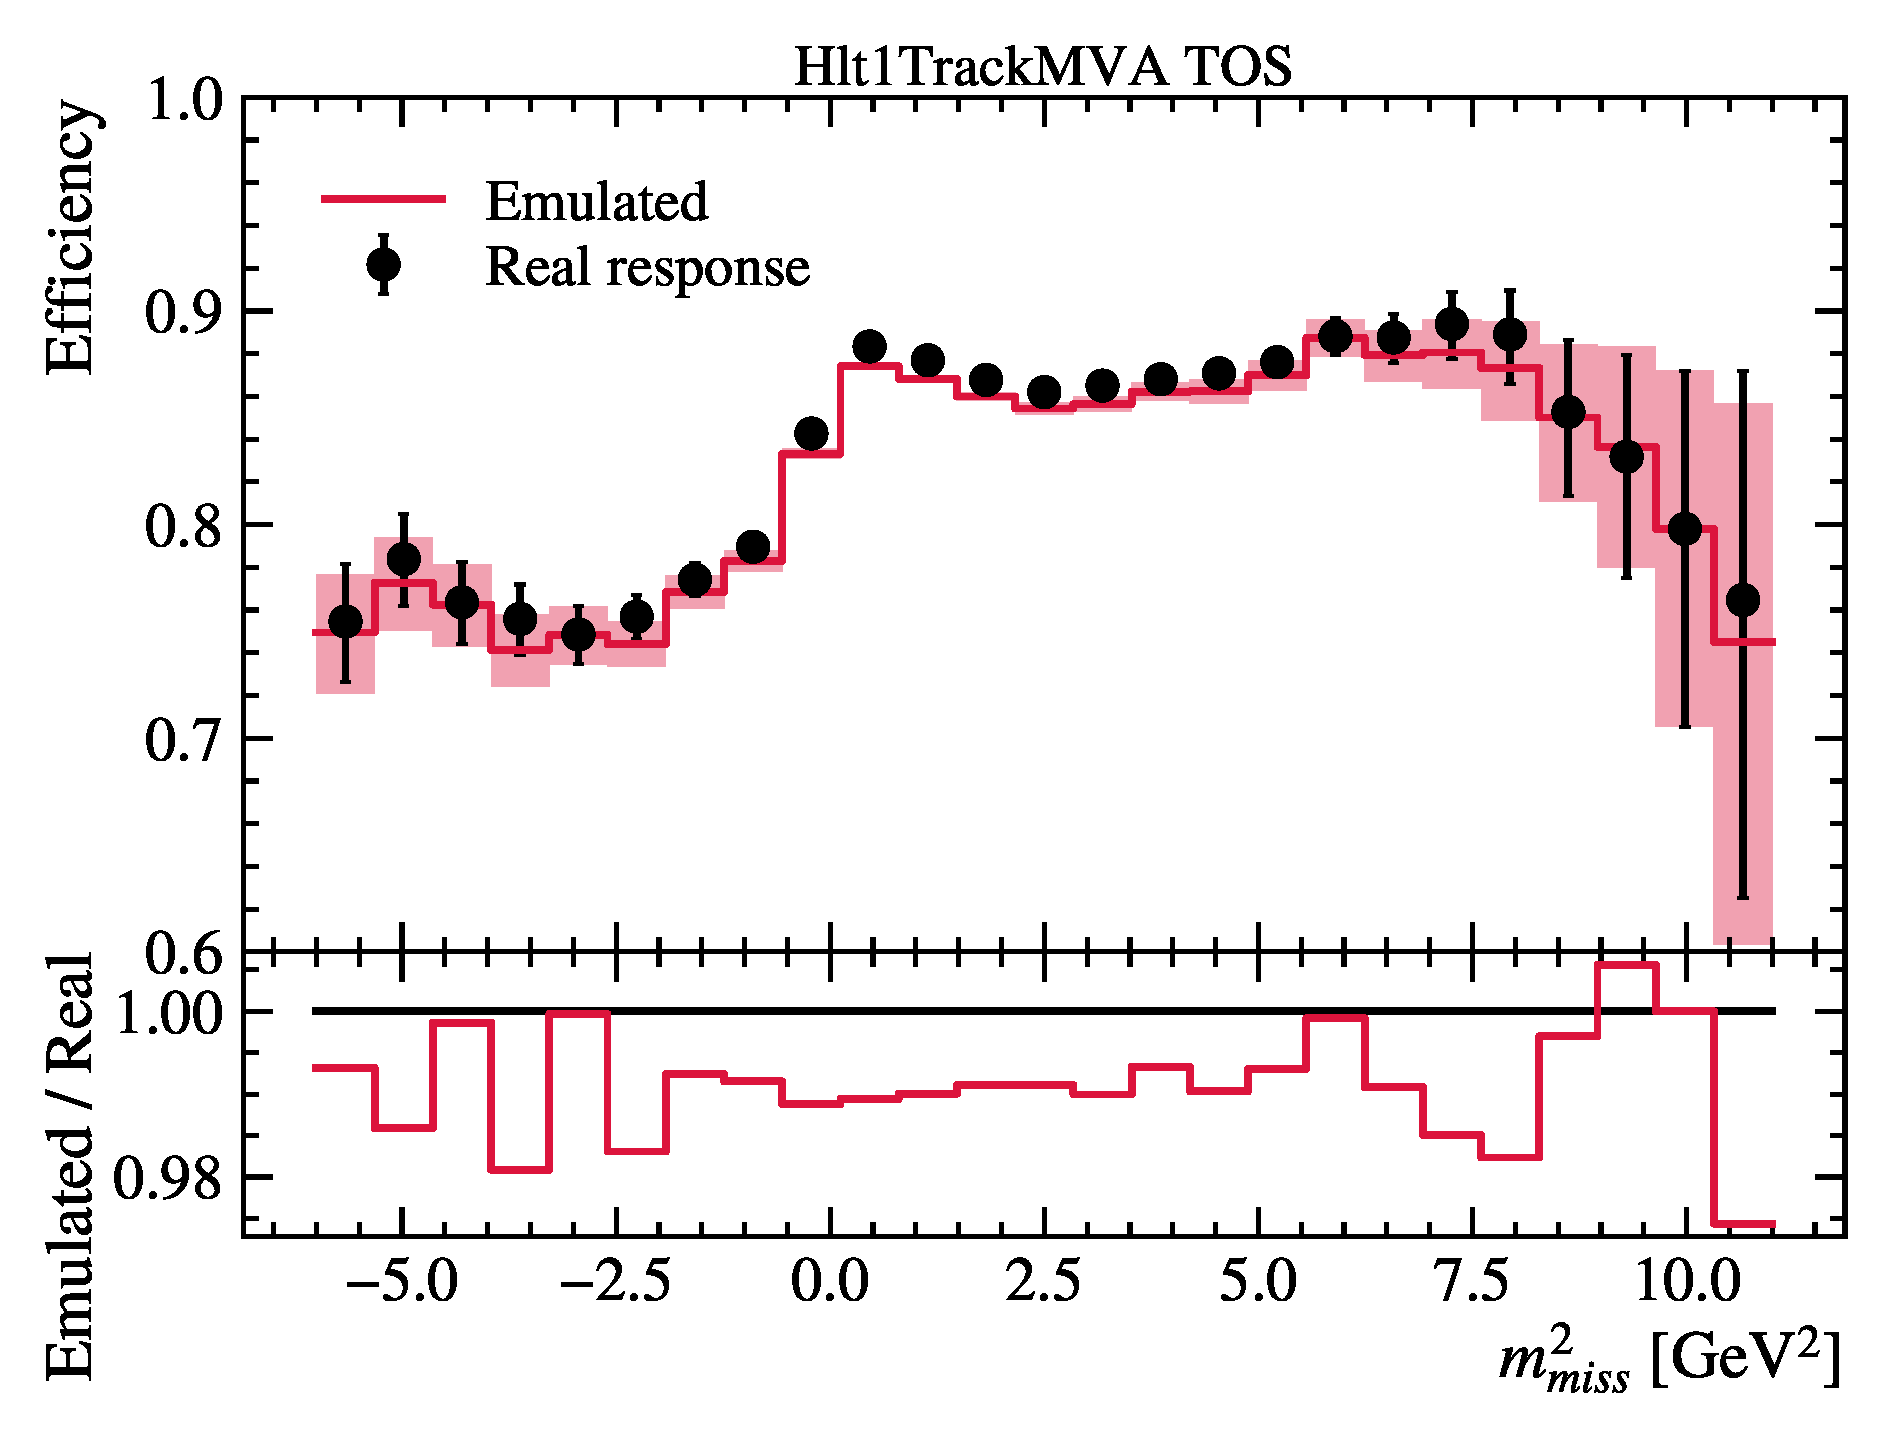
\includegraphics[width=0.32\textwidth]{
        ./figs-mc-emulation/emulate-hlt1/b_Hlt1TrackMVA_TOS_mmiss2.pdf
    }
    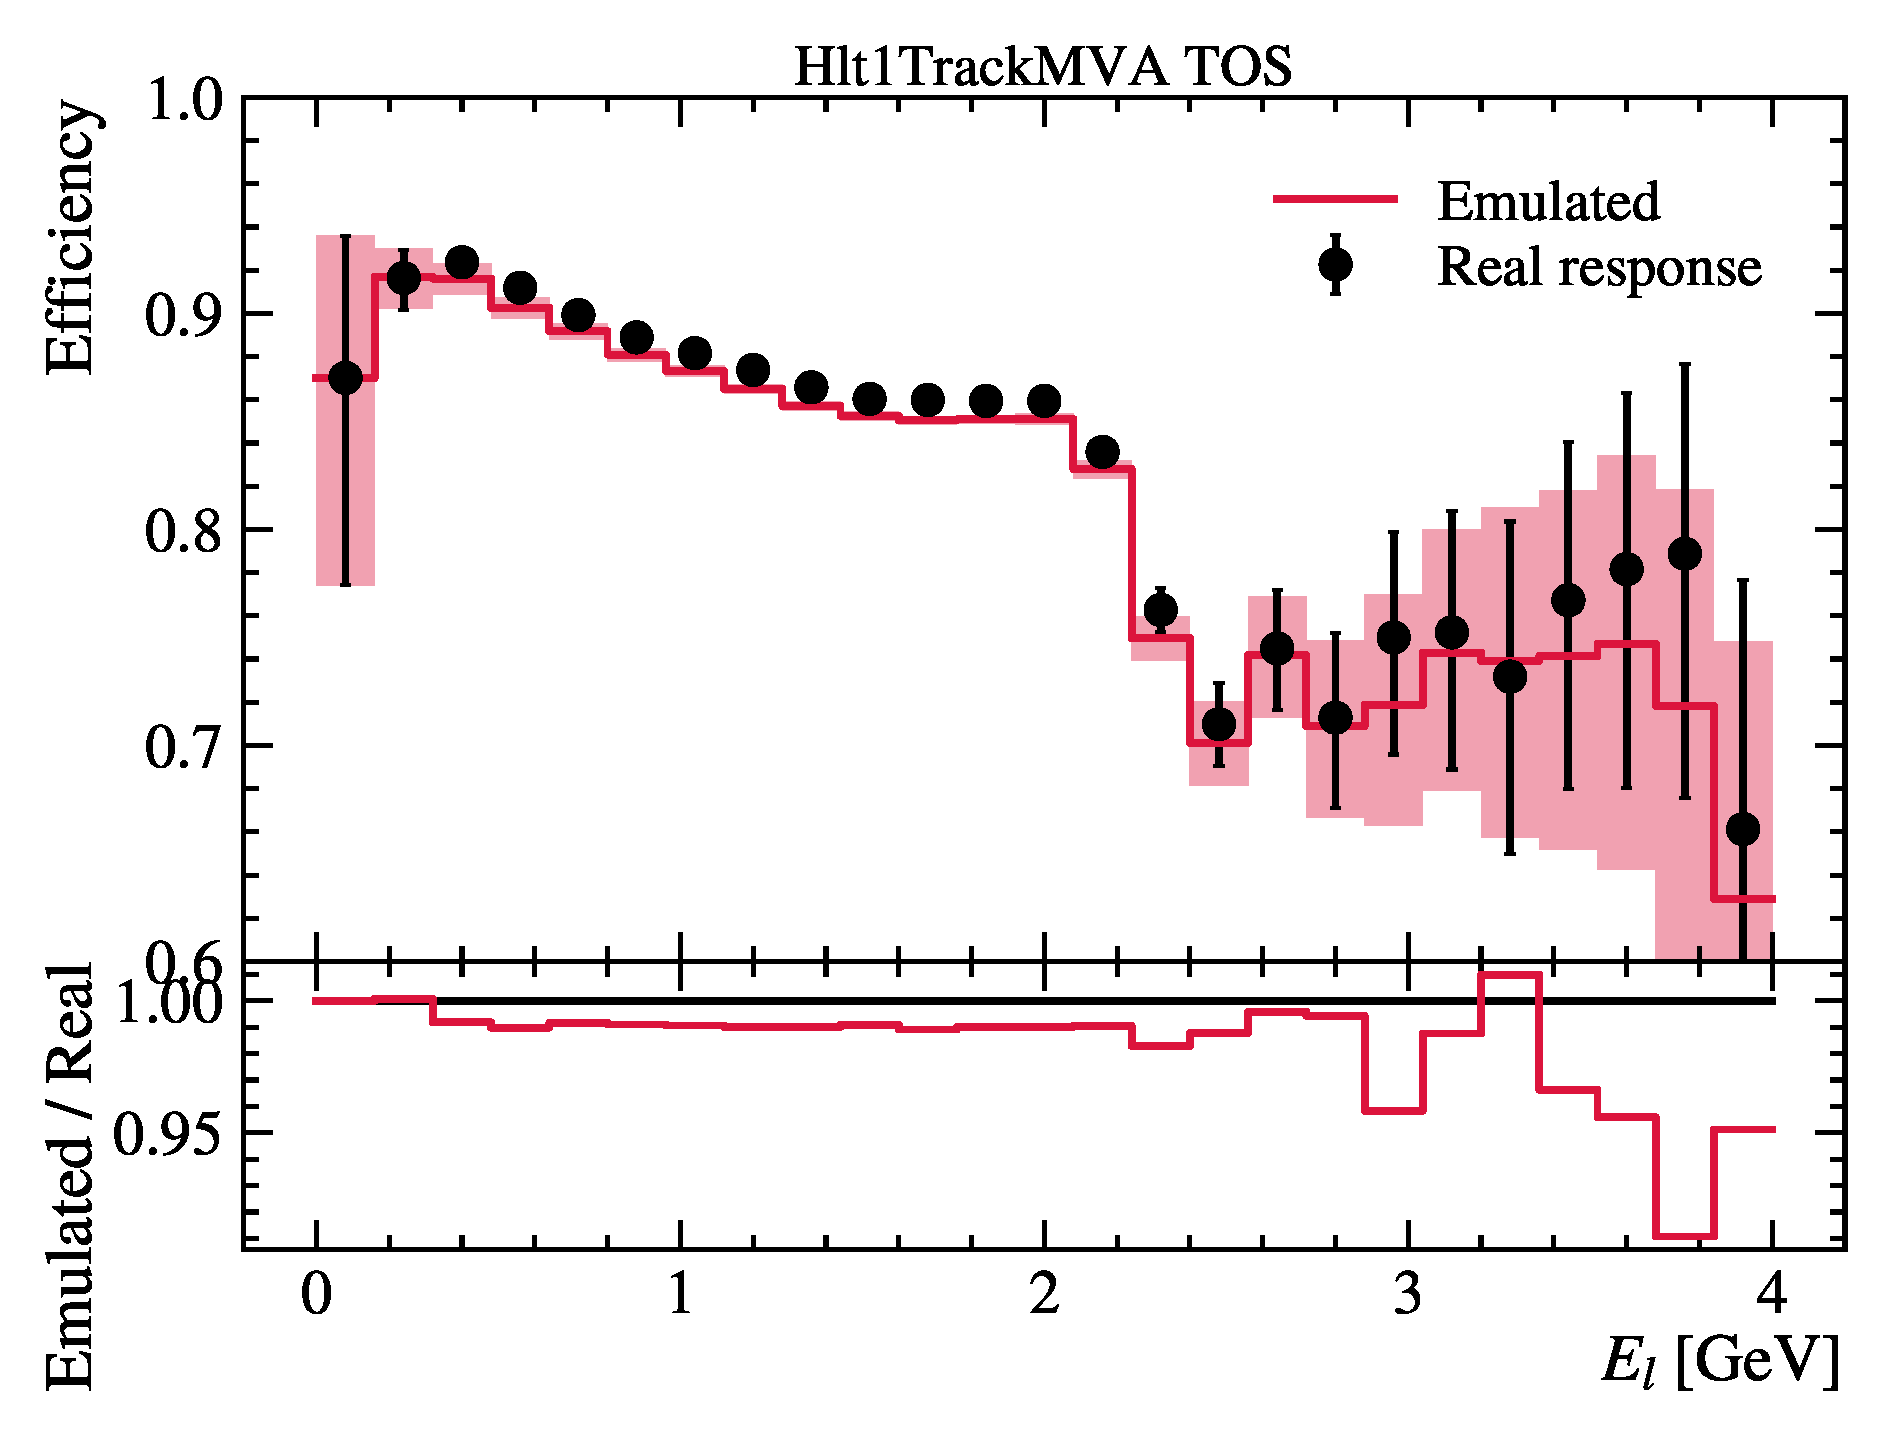
\includegraphics[width=0.32\textwidth]{
        ./figs-mc-emulation/emulate-hlt1/b_Hlt1TrackMVA_TOS_el.pdf
    }
    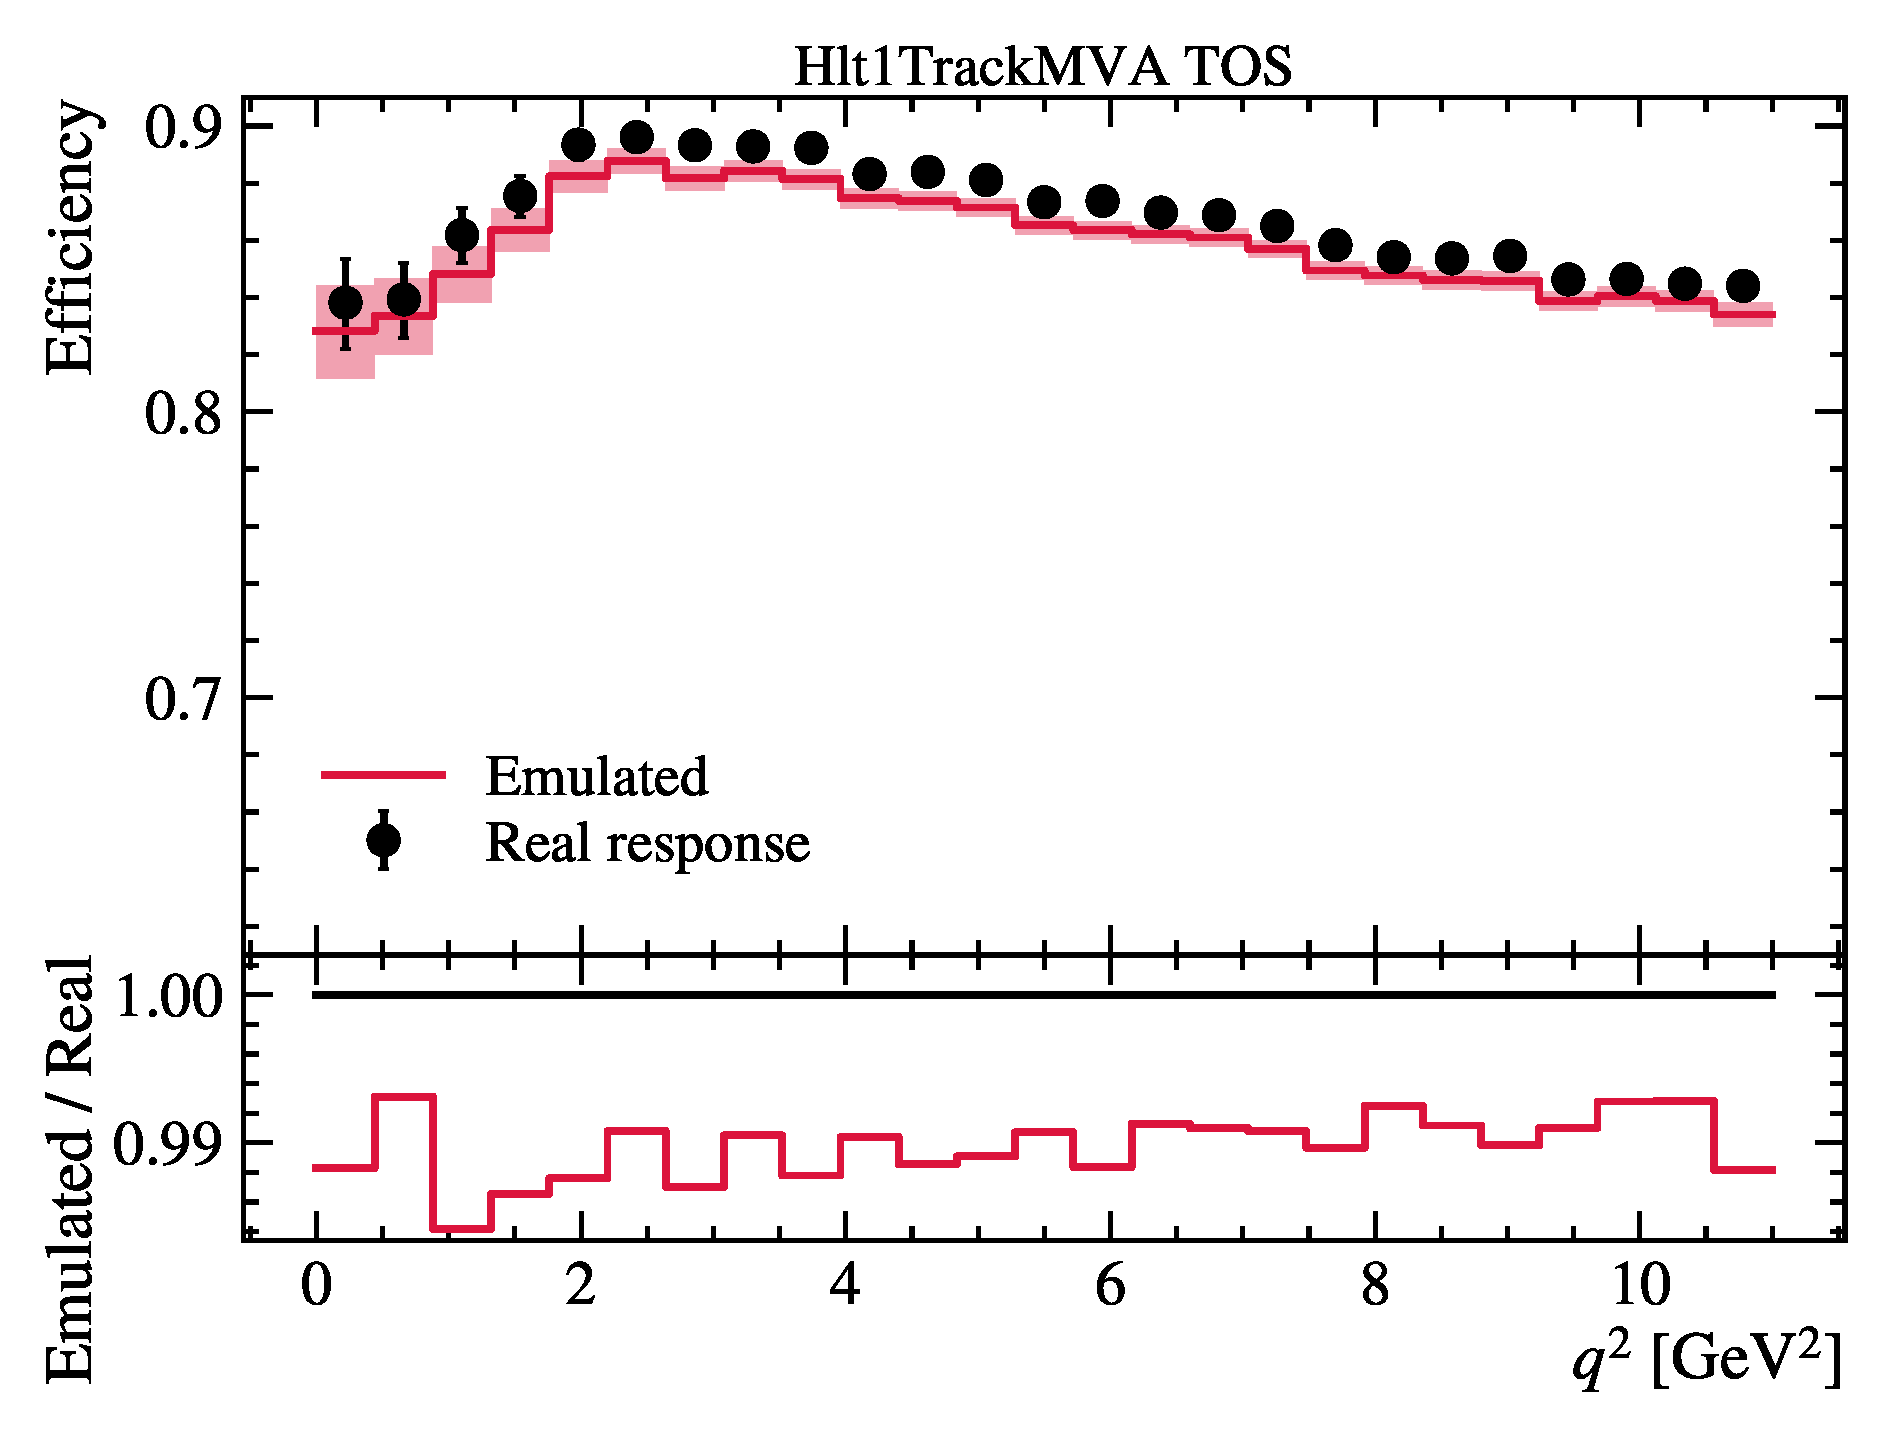
\includegraphics[width=0.32\textwidth]{
        ./figs-mc-emulation/emulate-hlt1/b_Hlt1TrackMVA_TOS_q2.pdf
    }

    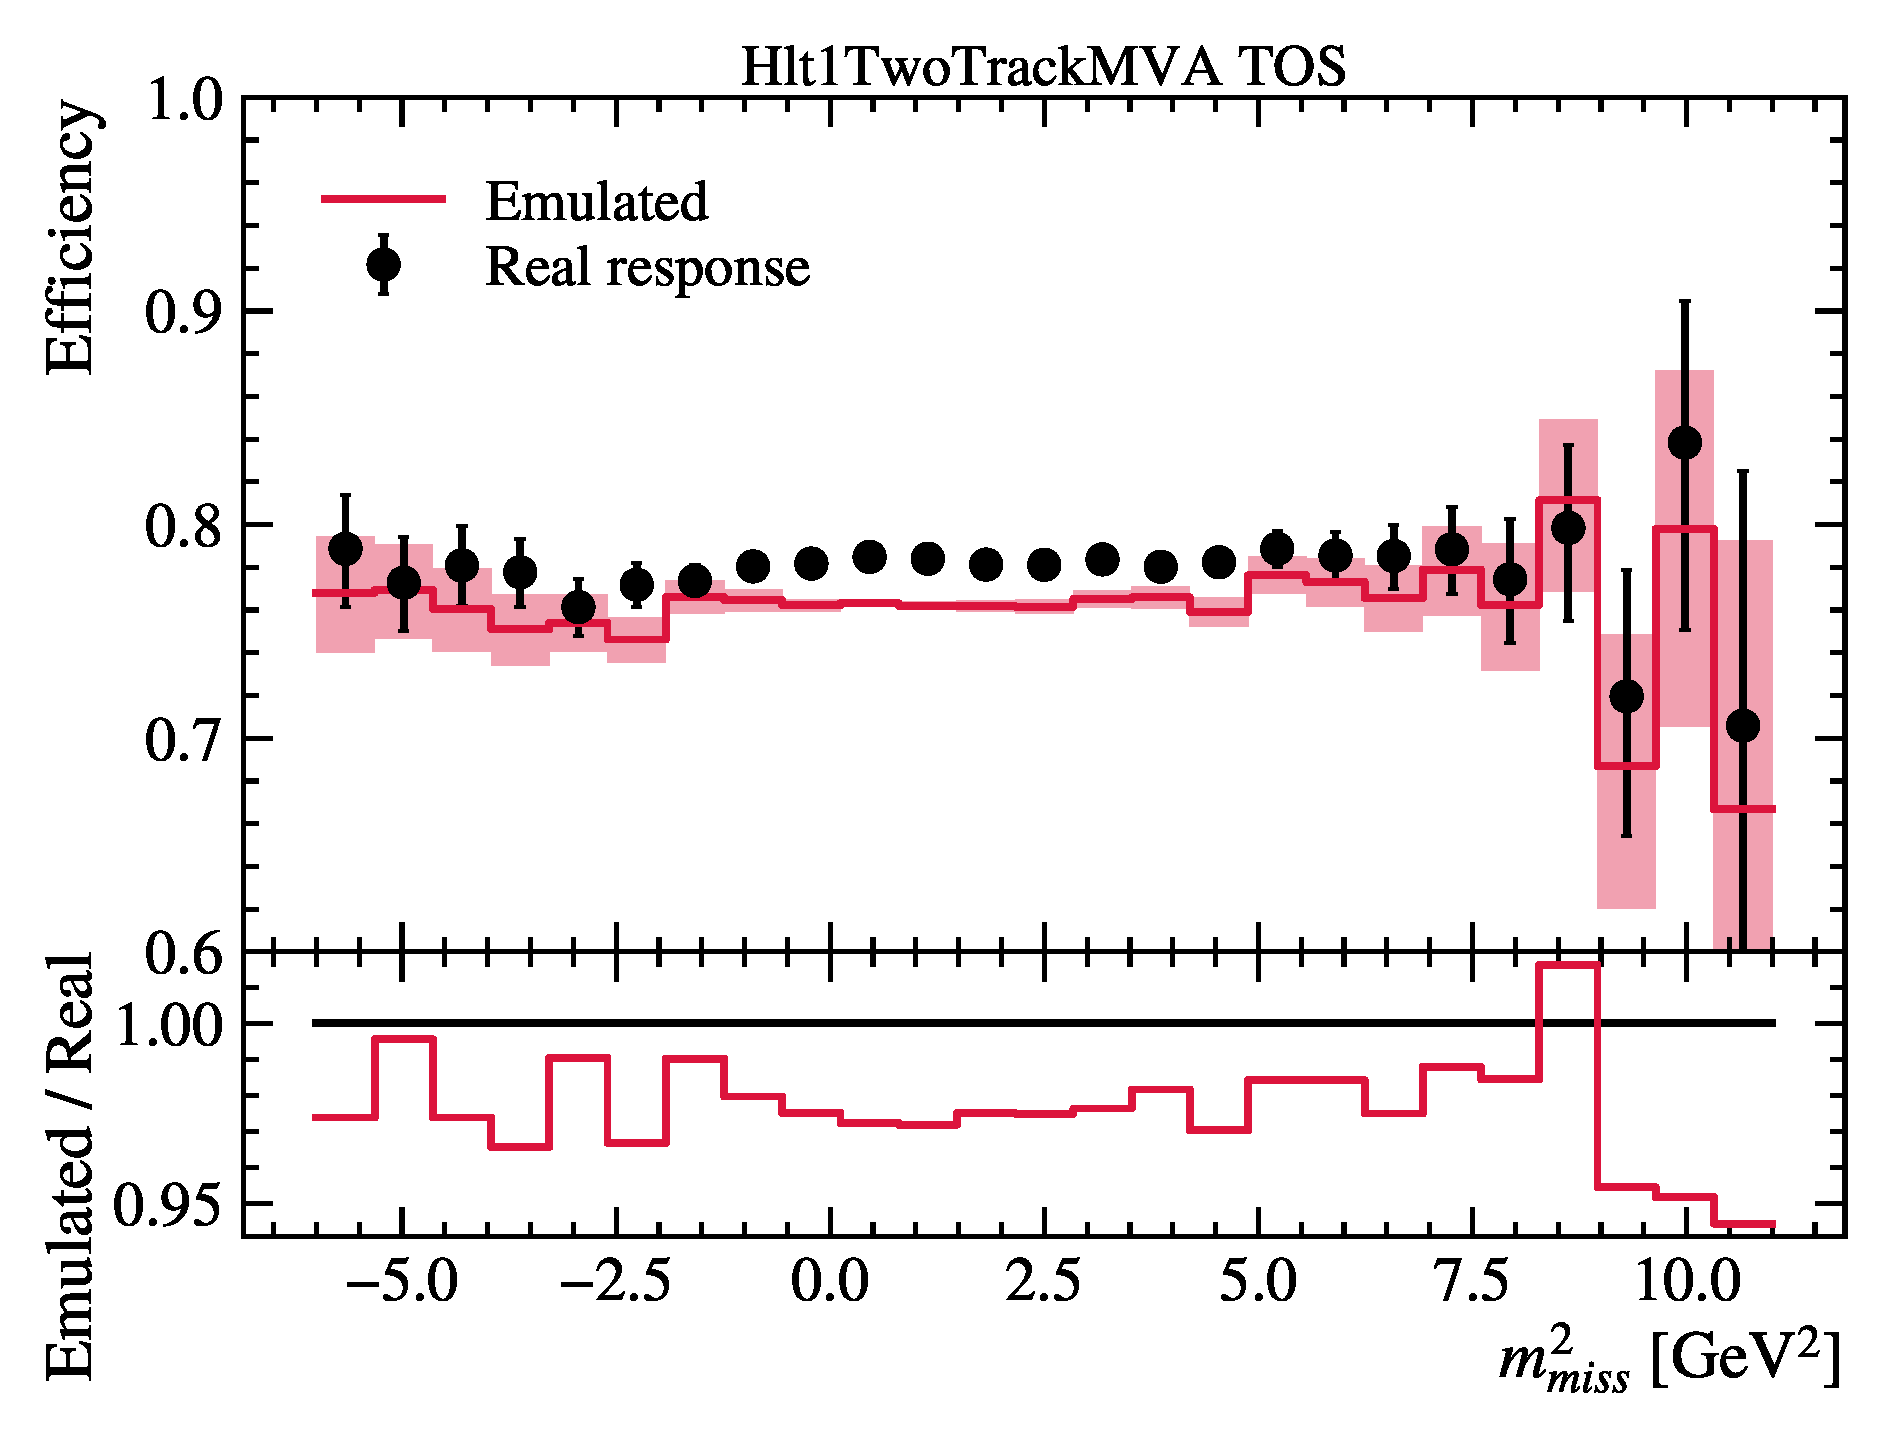
\includegraphics[width=0.32\textwidth]{
        ./figs-mc-emulation/emulate-hlt1/b_Hlt1TwoTrackMVA_TOS_mmiss2.pdf
    }
    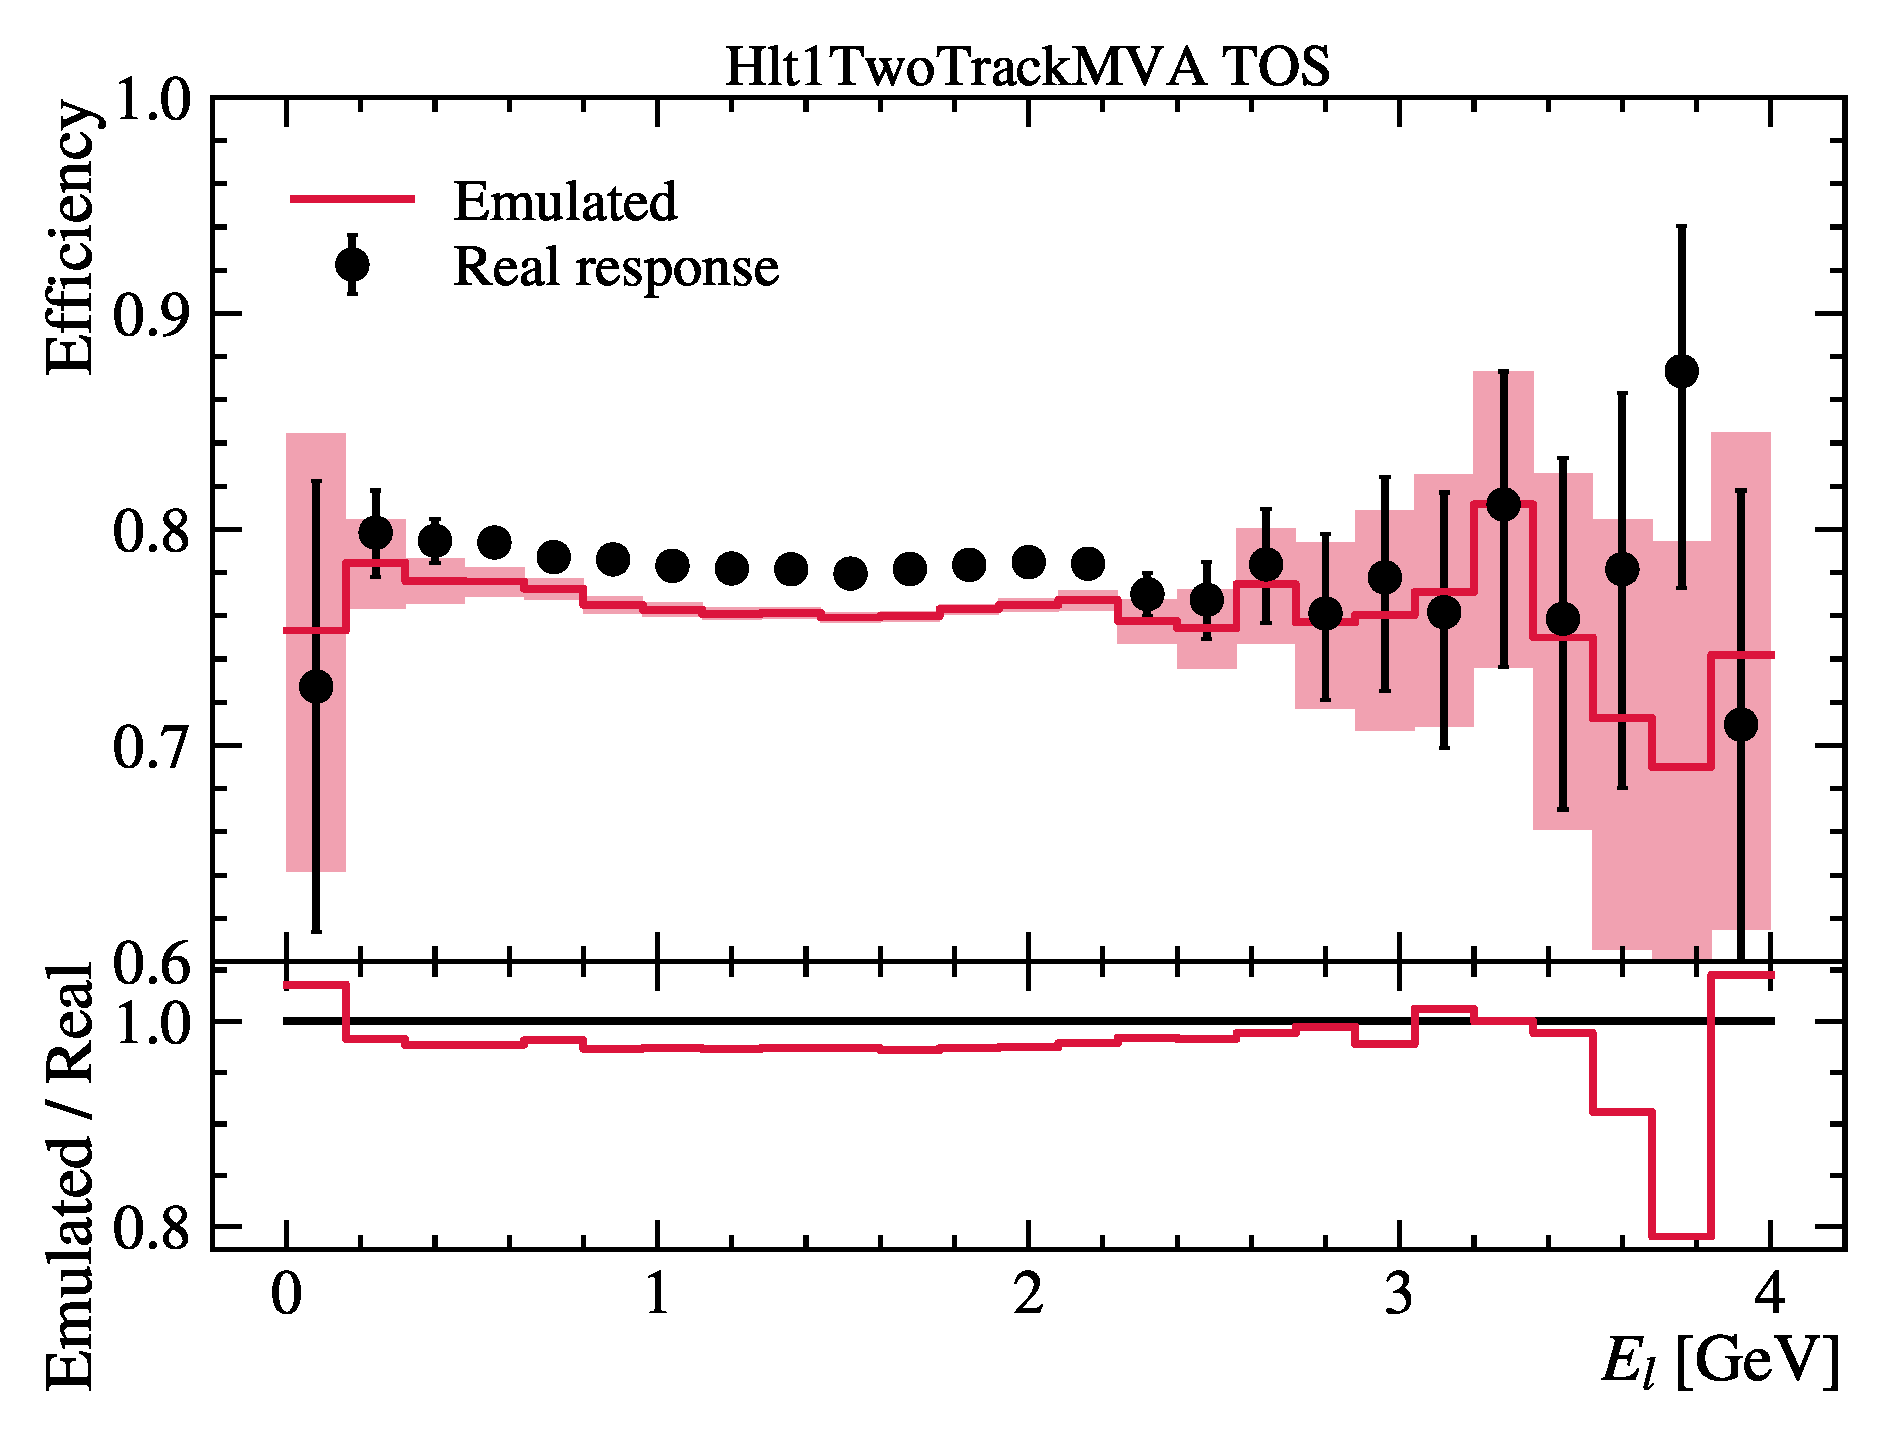
\includegraphics[width=0.32\textwidth]{
        ./figs-mc-emulation/emulate-hlt1/b_Hlt1TwoTrackMVA_TOS_el.pdf
    }
    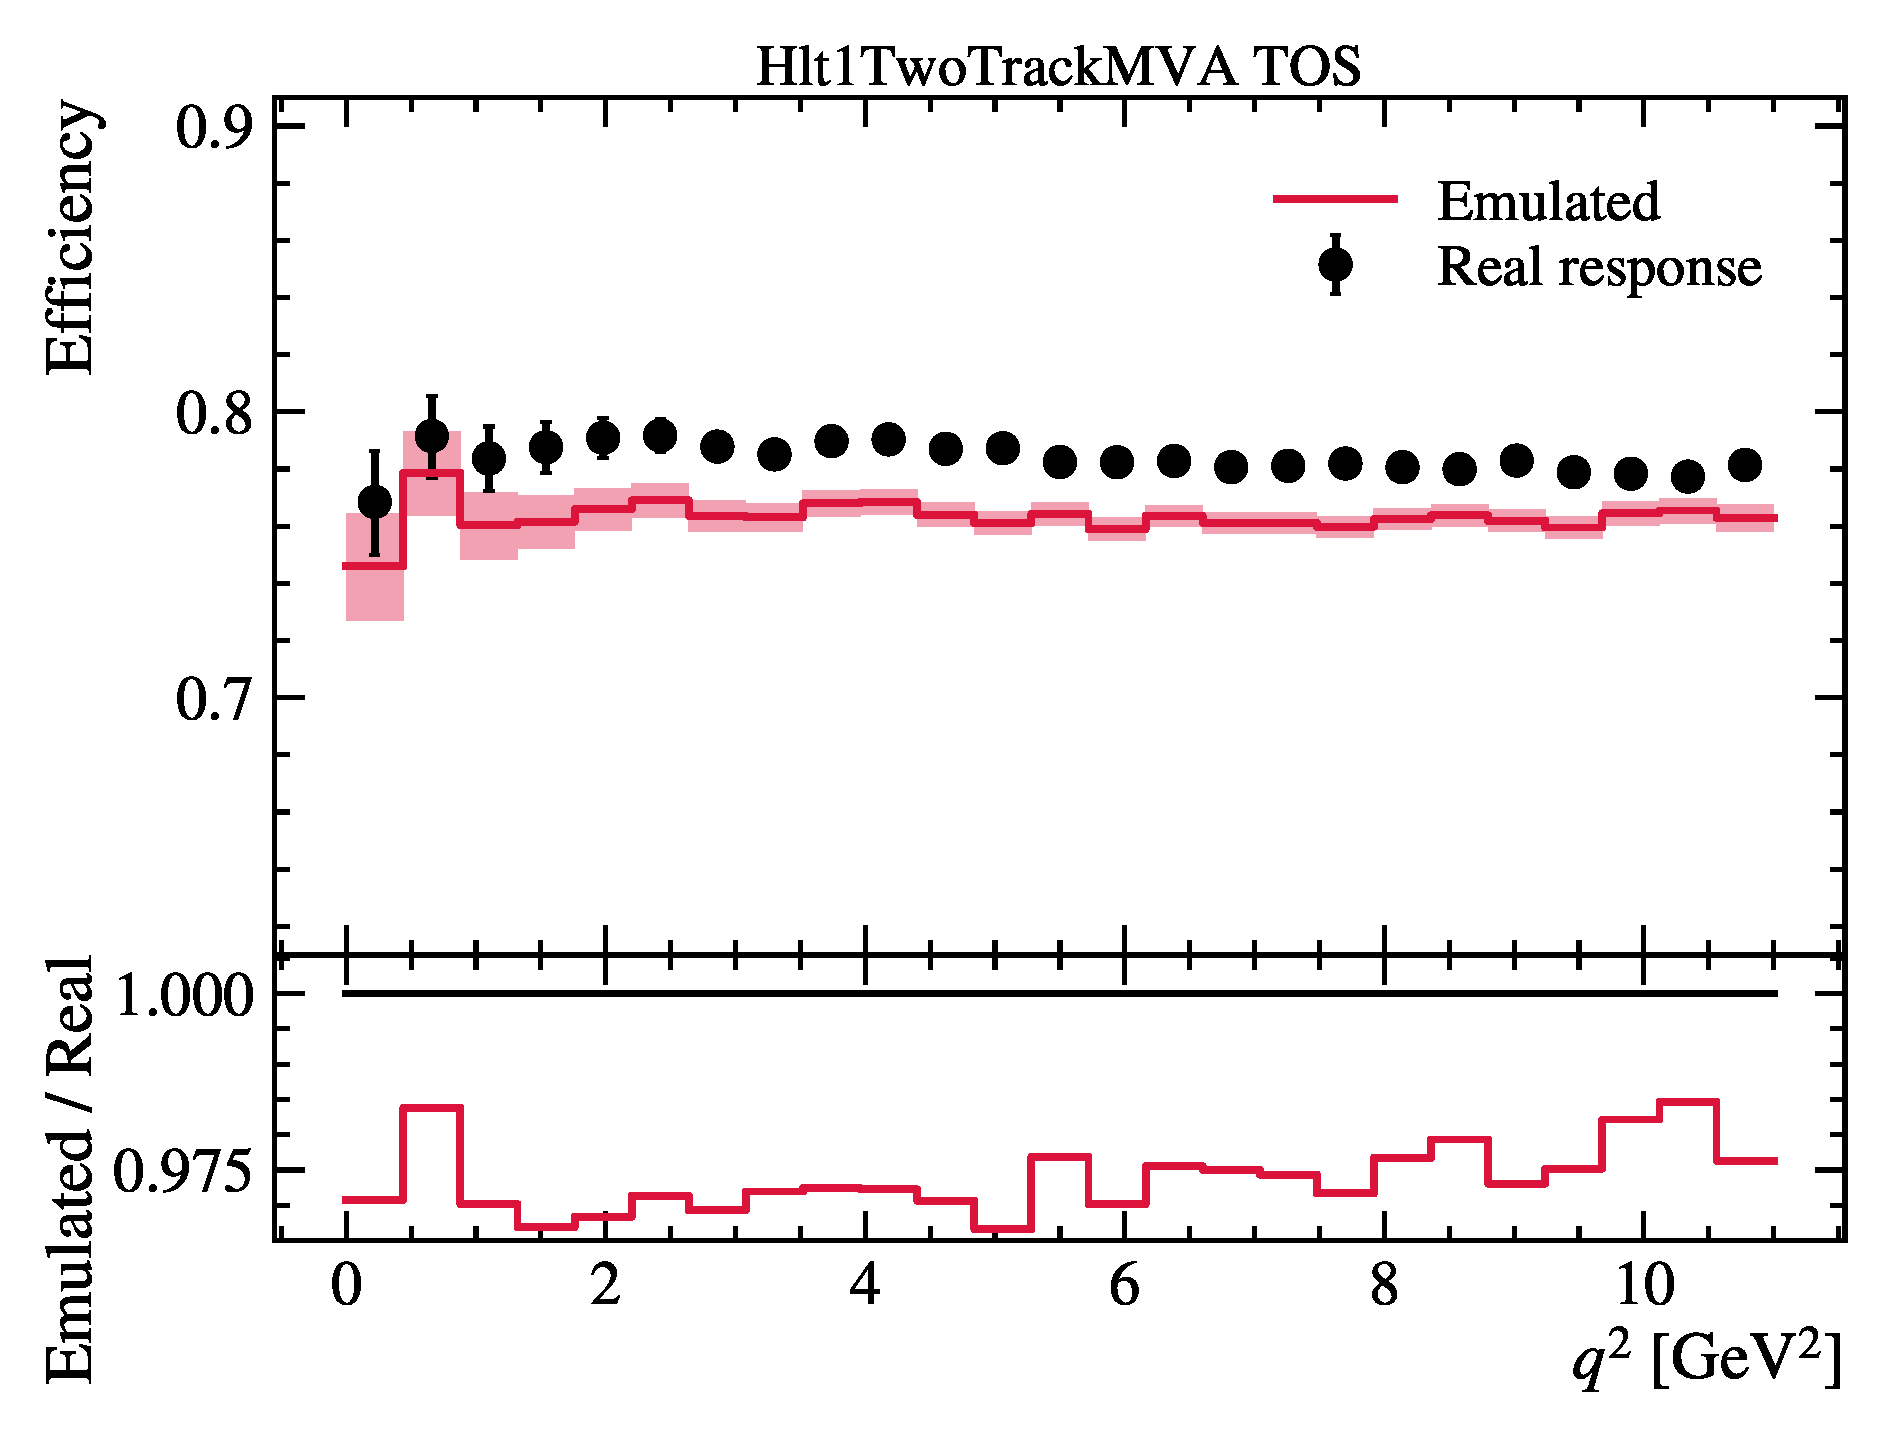
\includegraphics[width=0.32\textwidth]{
        ./figs-mc-emulation/emulate-hlt1/b_Hlt1TwoTrackMVA_TOS_q2.pdf
    }

    \caption{
        Emualted HLT1 triggers vs. real response in FullSim. For \Bp.
        The \smalltt{Hlt1TrackMVA} agree very well,
        whereas the \smalltt{Hlt1TwoTrackMVA} still has a constant,
        albeit small ($\sim\!2.25$\%), discrepancy.
    }
    \label{fig:hlt1-trackmva-emu}
\end{figure}

\begin{figure}[ht]
    \centering
    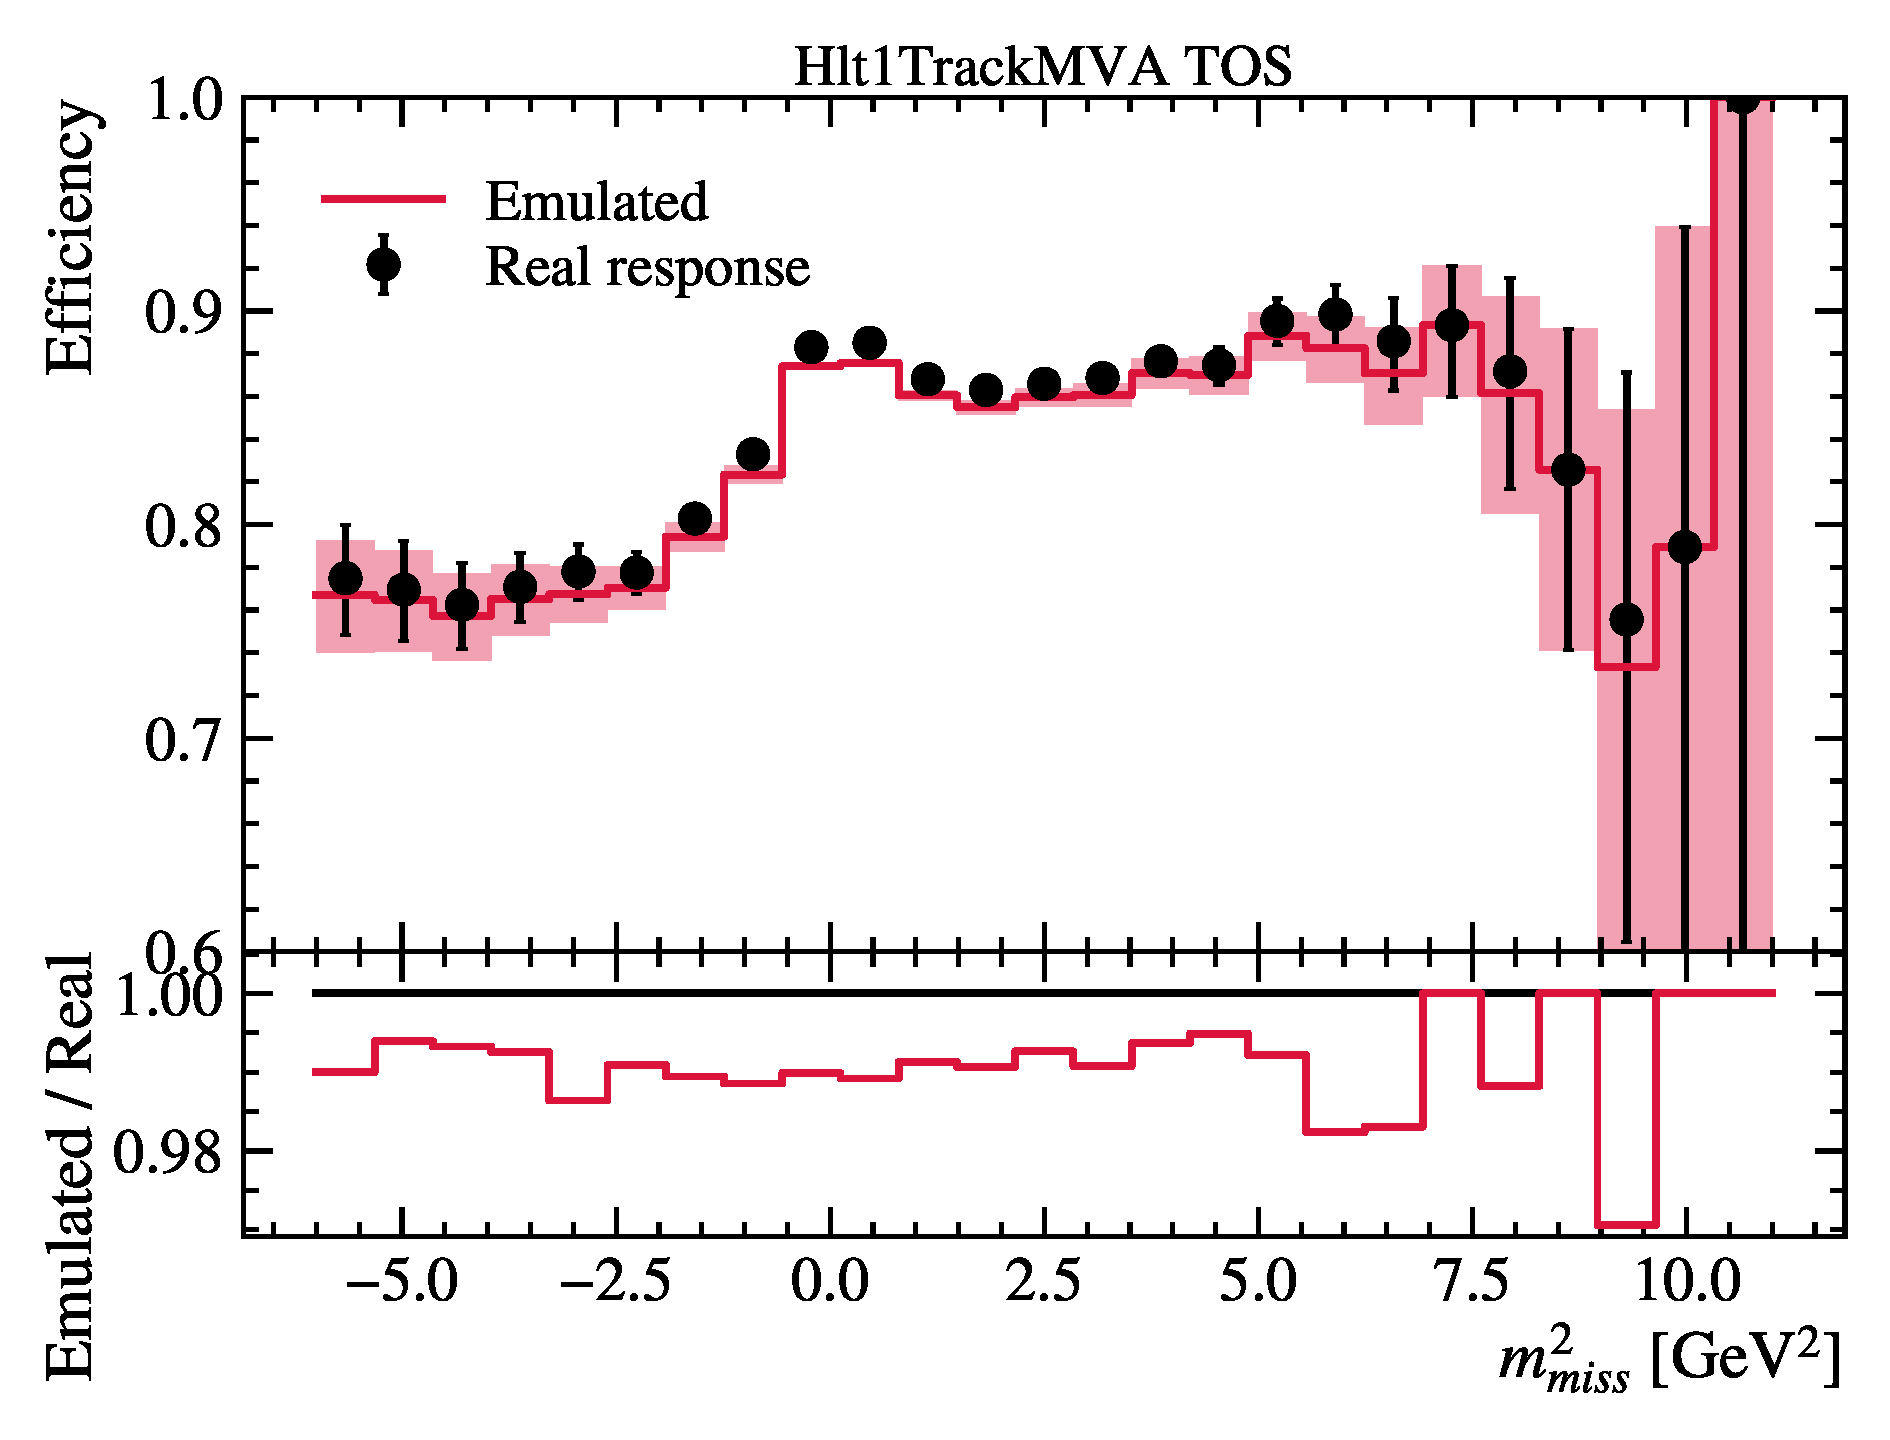
\includegraphics[width=0.32\textwidth]{
        ./figs-mc-emulation/emulate-hlt1/b0_Hlt1TrackMVA_TOS_mmiss2.pdf
    }
    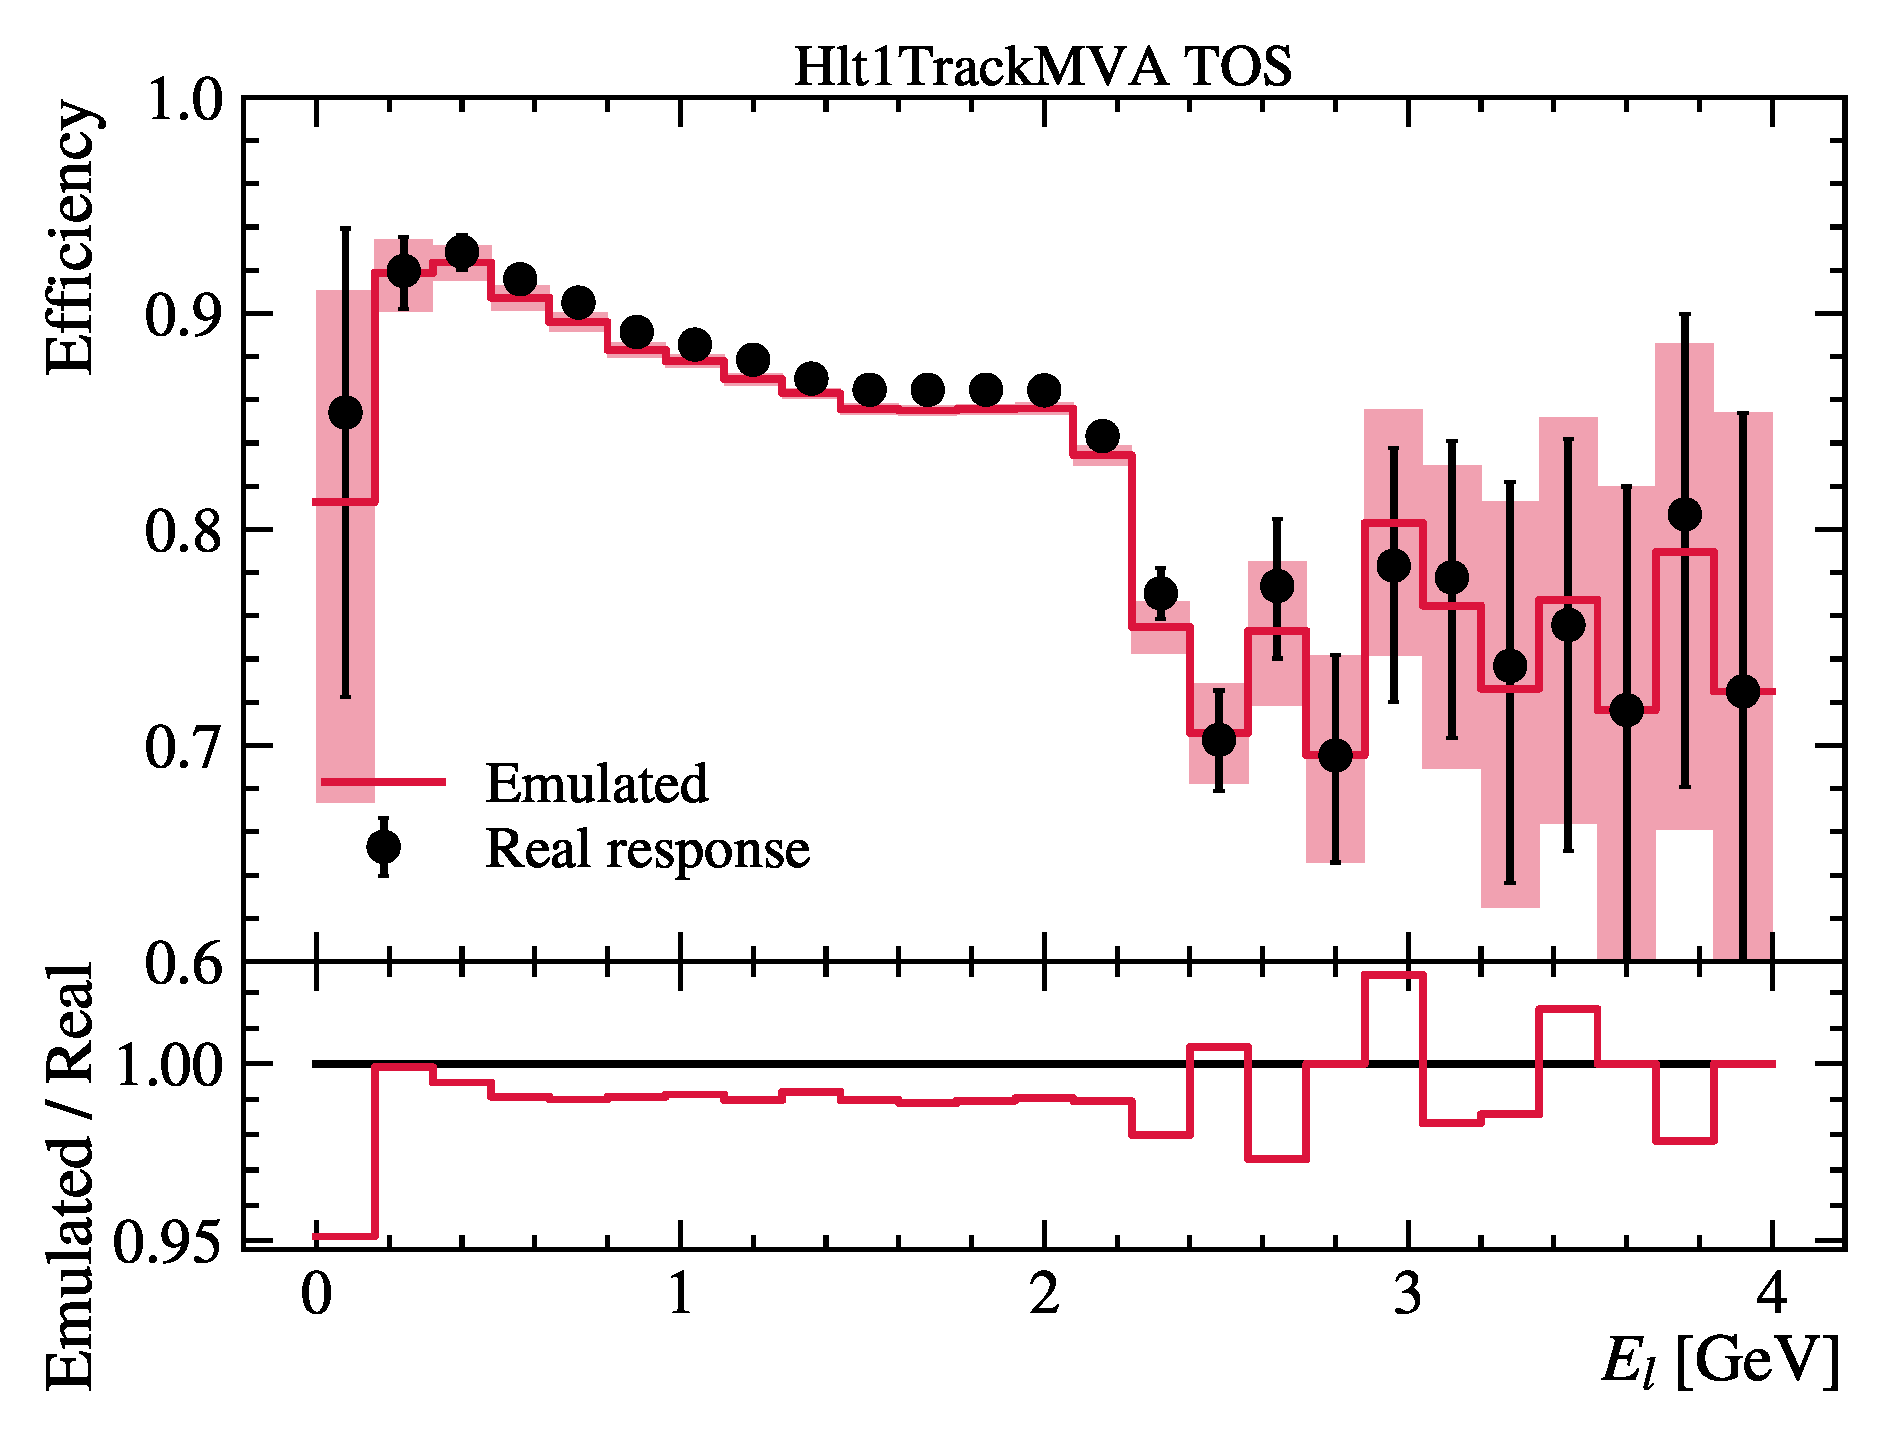
\includegraphics[width=0.32\textwidth]{
        ./figs-mc-emulation/emulate-hlt1/b0_Hlt1TrackMVA_TOS_el.pdf
    }
    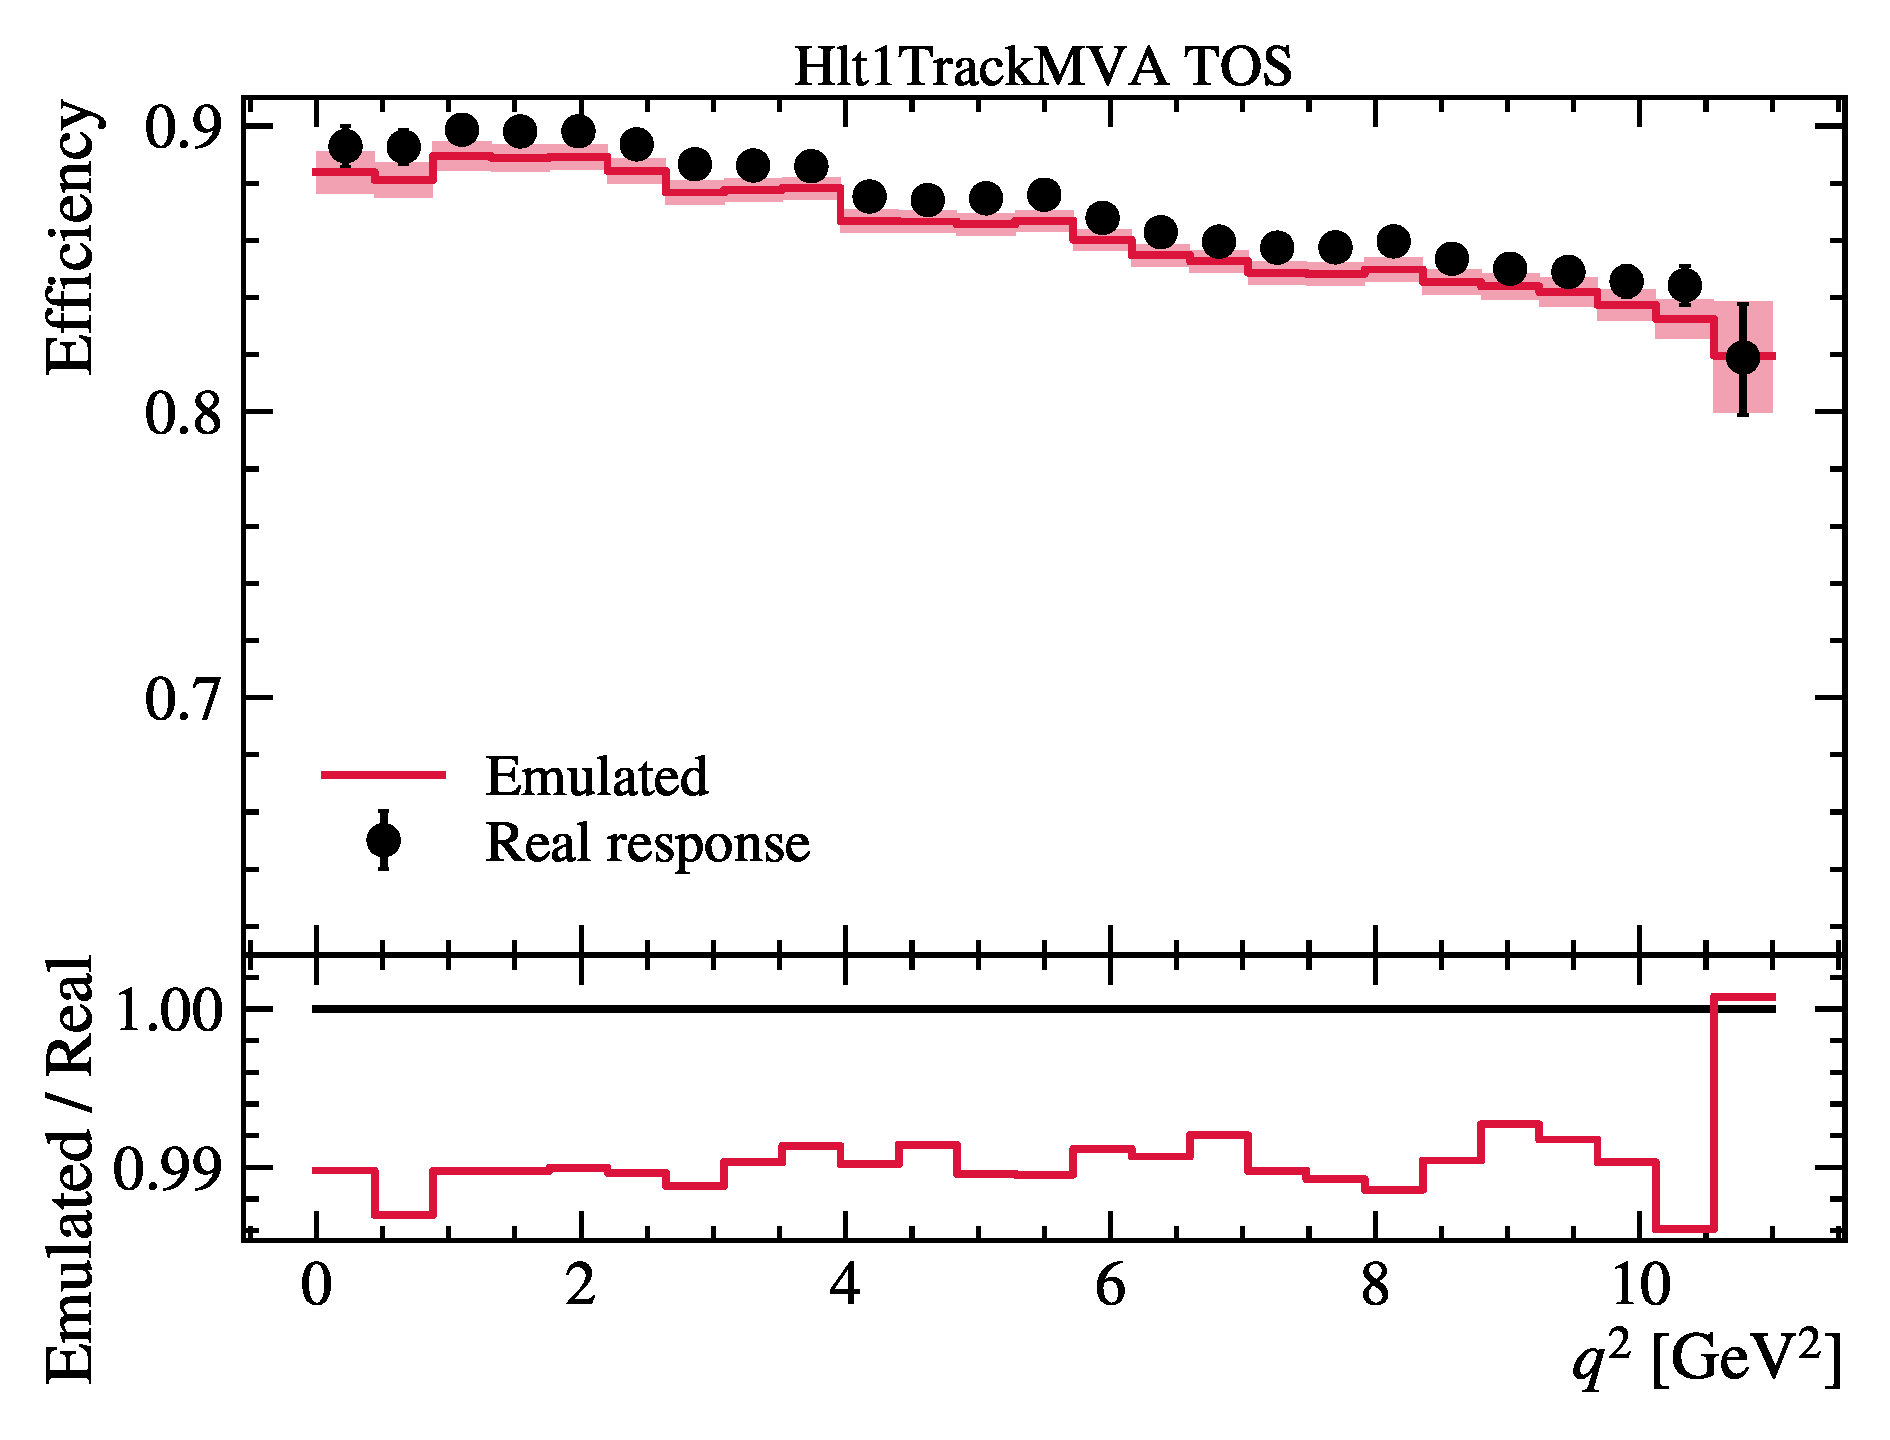
\includegraphics[width=0.32\textwidth]{
        ./figs-mc-emulation/emulate-hlt1/b0_Hlt1TrackMVA_TOS_q2.pdf
    }

    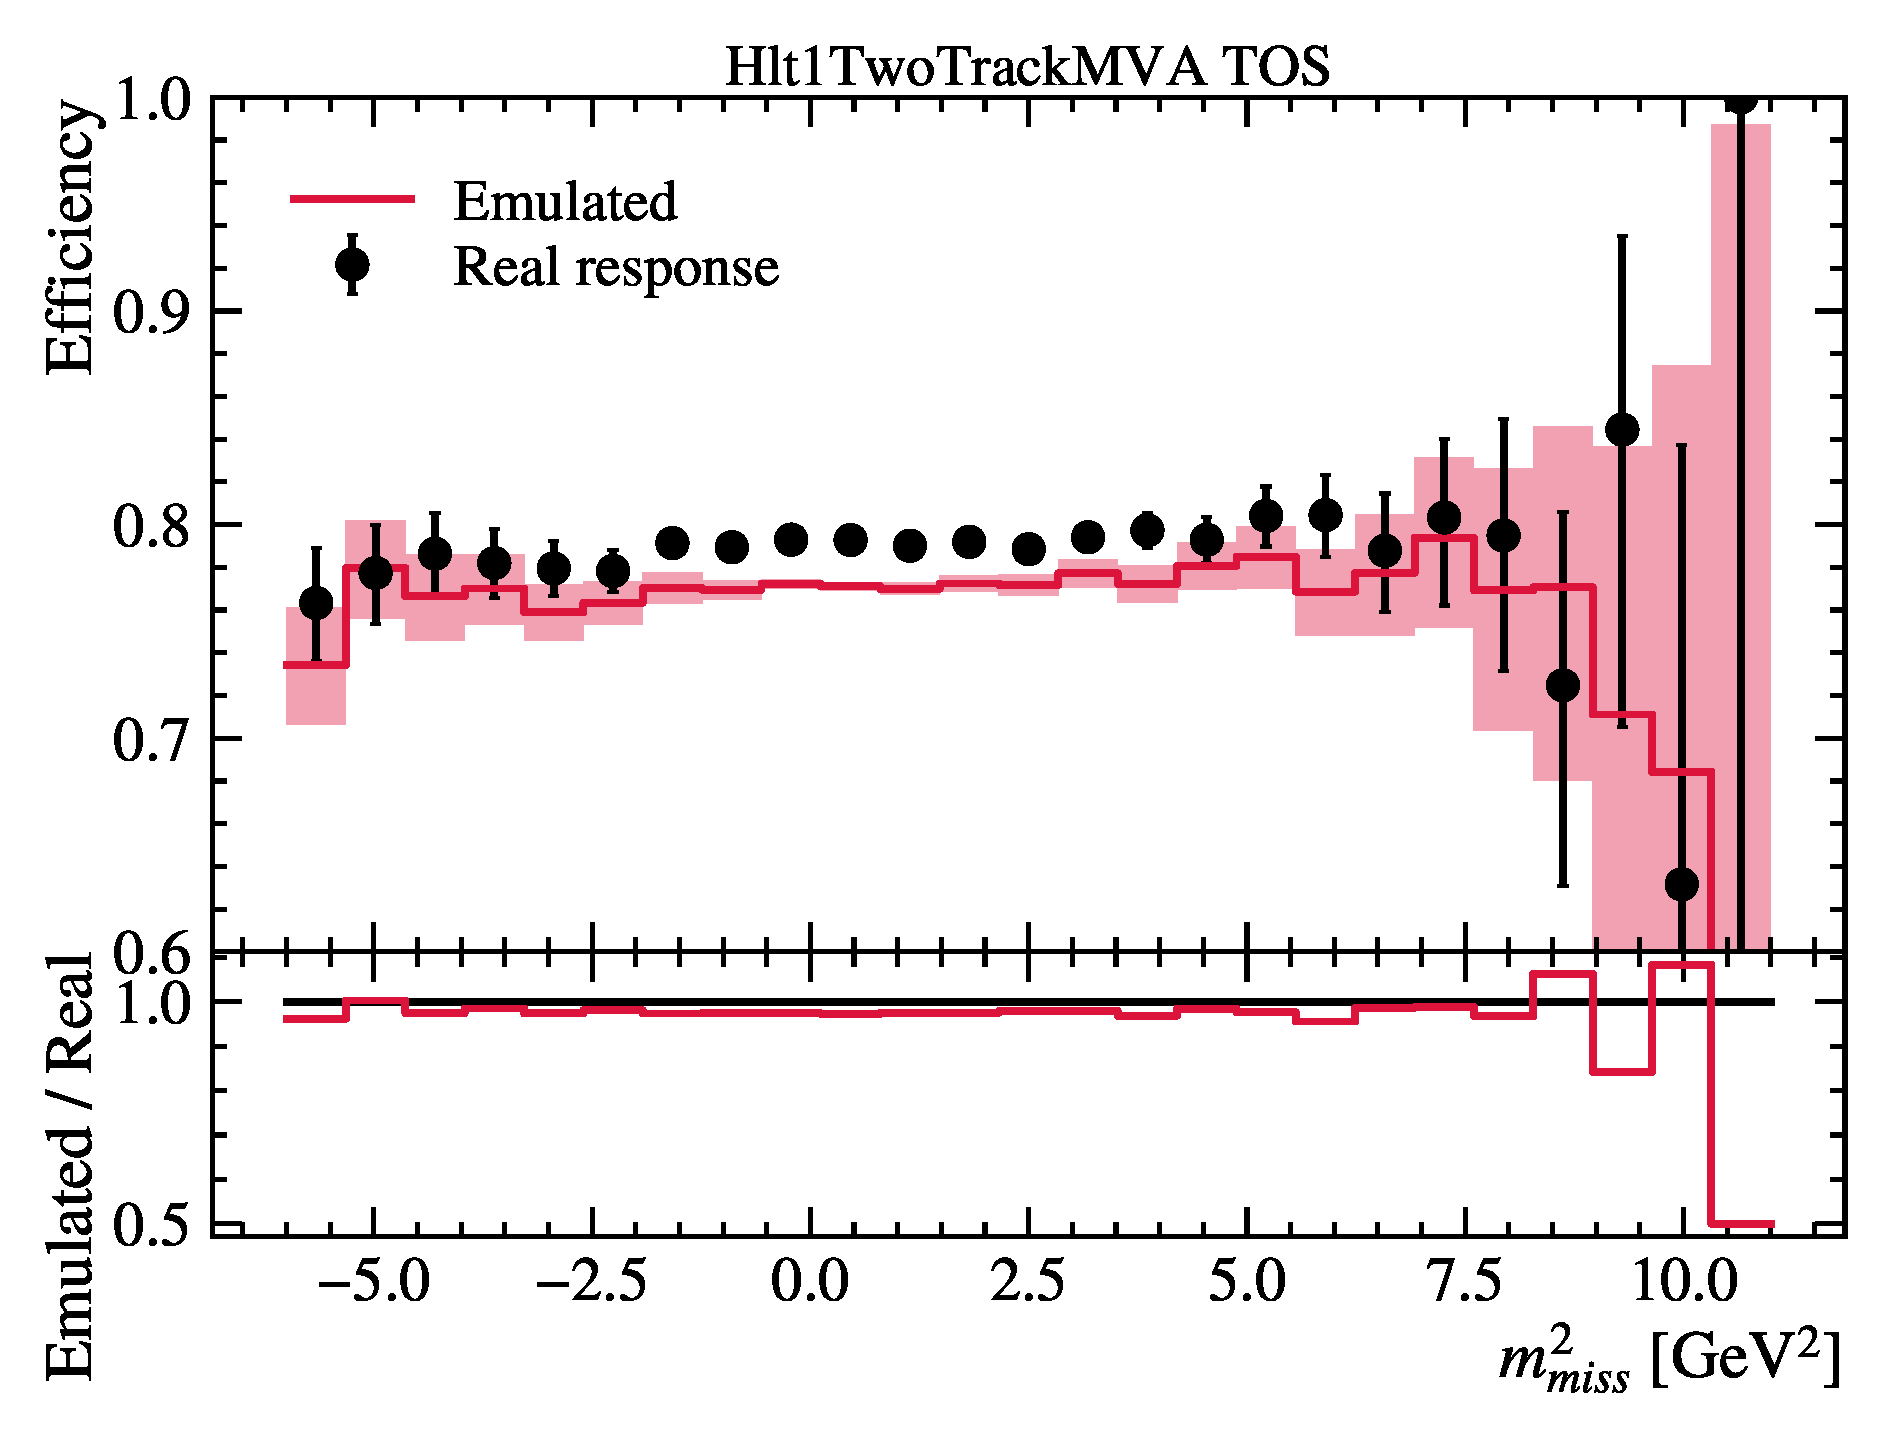
\includegraphics[width=0.32\textwidth]{
        ./figs-mc-emulation/emulate-hlt1/b0_Hlt1TwoTrackMVA_TOS_mmiss2.pdf
    }
    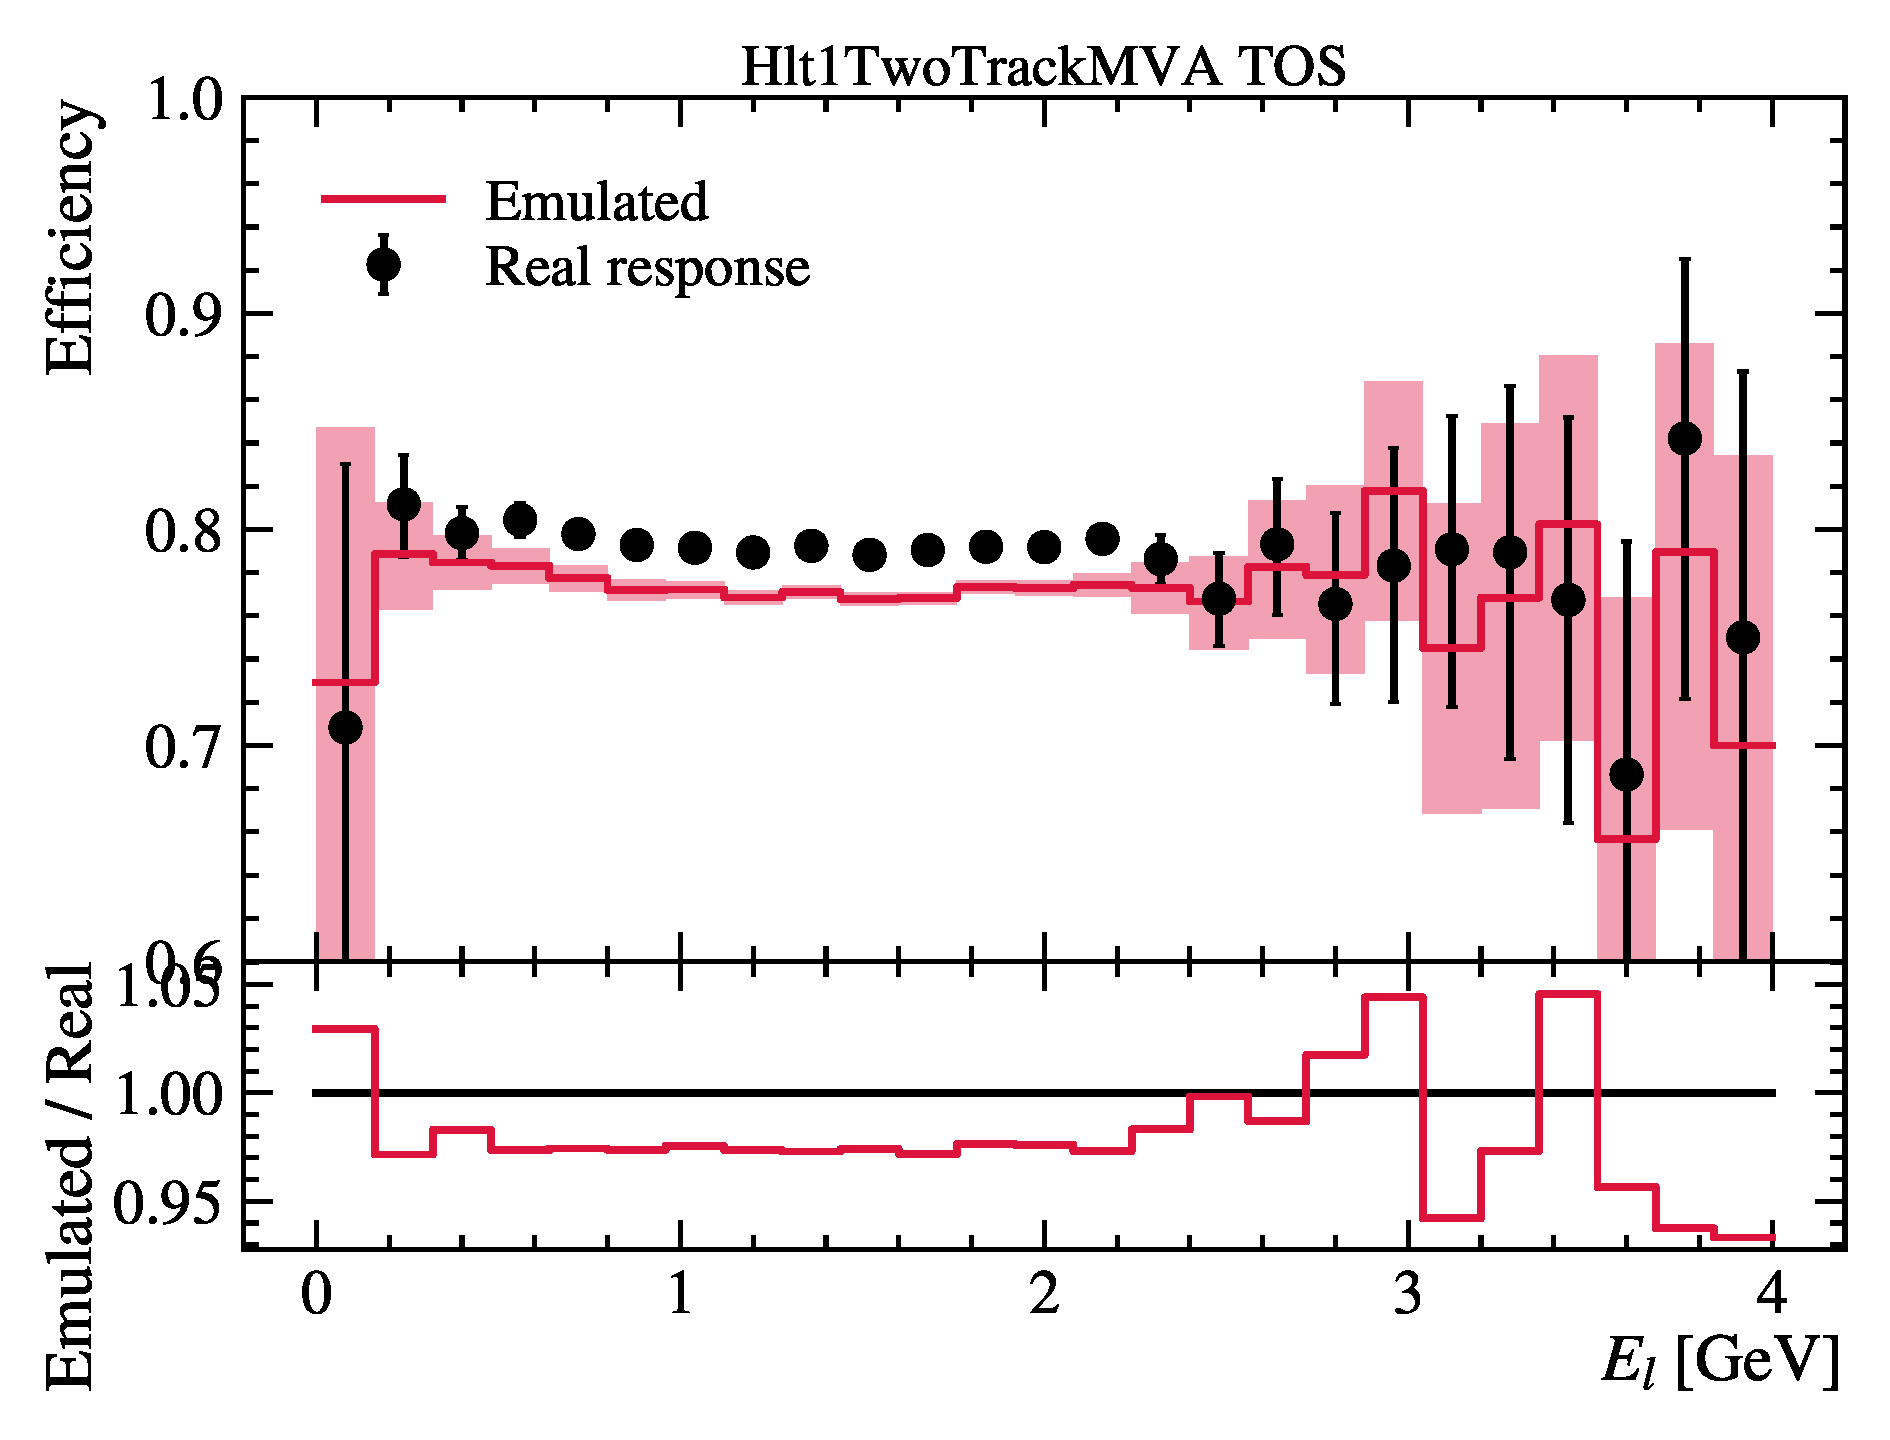
\includegraphics[width=0.32\textwidth]{
        ./figs-mc-emulation/emulate-hlt1/b0_Hlt1TwoTrackMVA_TOS_el.pdf
    }
    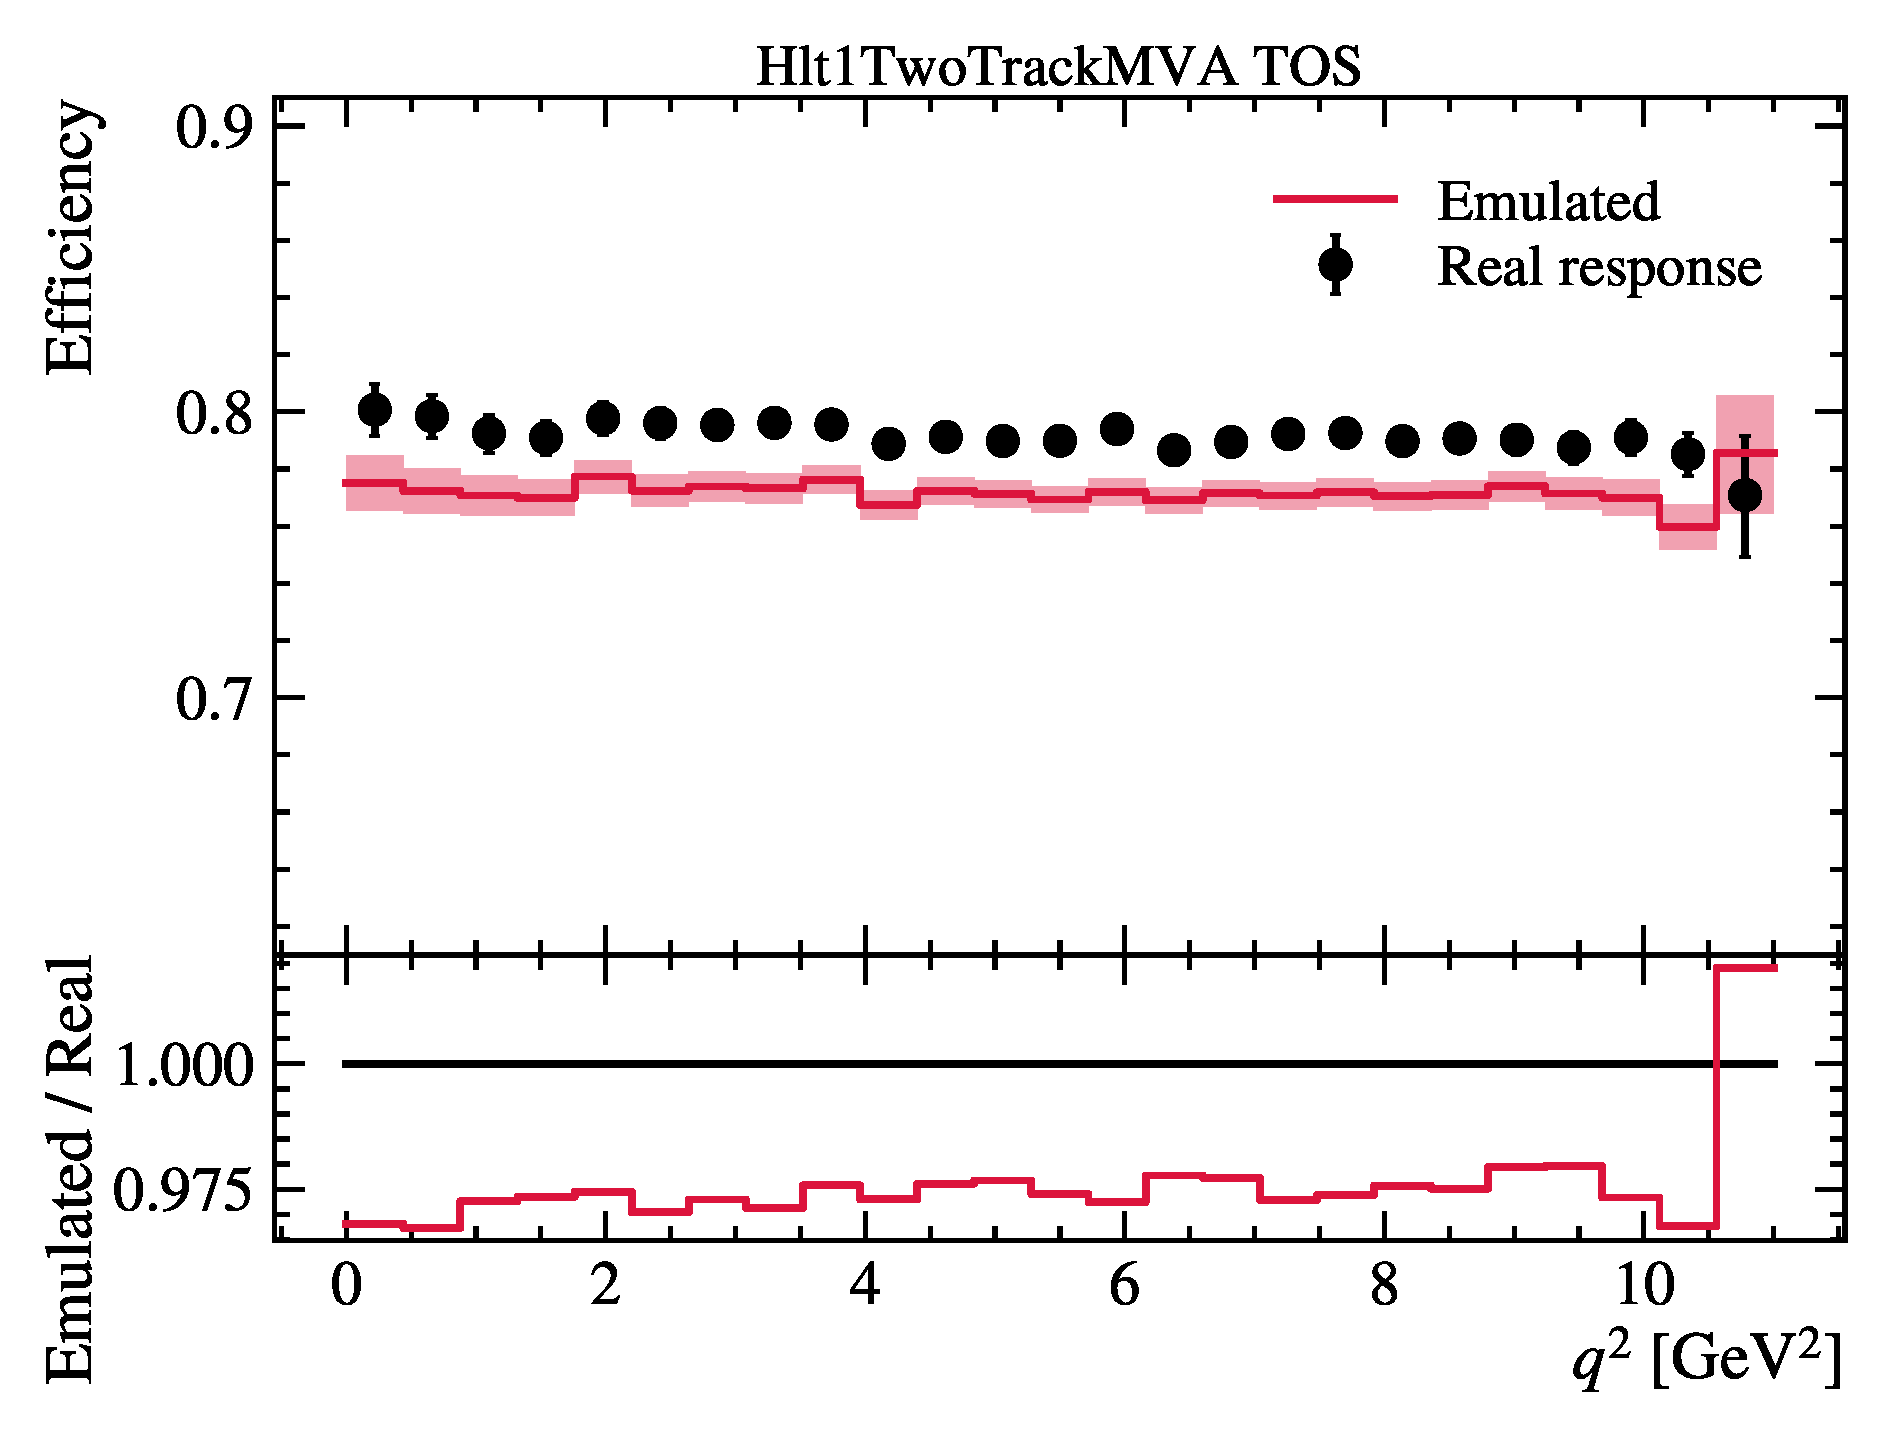
\includegraphics[width=0.32\textwidth]{
        ./figs-mc-emulation/emulate-hlt1/b0_Hlt1TwoTrackMVA_TOS_q2.pdf
    }

    \caption{
        Emualted HLT1 triggers in \Bz have similar level of agreement to real
        response compared to that of \Bp.
    }
    \label{fig:hlt1-twotrackmva-emu}
\end{figure}


\subsection{Emulation of \texttt{Hlt2XcMuXForTauB2XcMu}}

The selected \B is required to TOS on \smalltt{Hlt2XcMuXForTauB2XcMu}.
All selection variables listed in \cref{tab:cut-hlt2} are available in the
selection procedure so these cuts are applied directly.


\section{Particle identification emulation}
\label{ref:mc-emulation:pid}

Tracker-Only MC has RICH and calorimeters, sub-detectors responsible for
particle identification (PID), set to passive material, thus no PID cut can be
applied directly on MC.
Therefore, PID cuts for MC are emulated as efficiencies (binned in some
variables, typically $p$, $\eta$, and nTracks) and applied as weights.

Most of PID efficiencies are obtained with \pidcalib, an official LHCb package
which provide PID efficiencies evaluated at user-specified cuts on
officially produced PID samples from real data with a customizable binning.
the PID samples are highly enriched in charged $K, \pi, p, e, \mu$, and are
obtained from reconstructed $K_s^0 \rightarrow \pip \pim$,
$\Lambda_c^0 \rightarrow p^+ \pim$,
$\Dstarp \rightarrow \Dz (\rightarrow \Km \pip) \pip$,
$\jpsi \rightarrow \mup \mun$, and
$\Bp \rightarrow \jpsi (\rightarrow e^+ e^-) \Kp$ data samples.
These samples are shown to have high purity in \cite{LHCb-DP-2012-003}.

It is worth noting that \pidcalib does not populate under and overflow bins,
therefore a custom binning scheme, extended from the official scheme, is used
for \pidcalib efficiencies to
avoid introducing unnecessarily tight kinematic cuts\footnote{
    Still, a momentum upper bound cut is applied, which is
    listed in \cref{tab:offline-cut-common}.
}.
Another thing to note is that the $e$ sample lacks \UBDT, so an
incremental \UBDT efficiency is obtained from true $e$ reconstructed as \muon
in 2016 $D^*\mu$ MC.

The skim selection as listed in \cref{tab:skim-cut}
contains a \ProbNN{$K$} PID cut on a track of unknown particle type.
To emulate this cut, the PID efficiencies from all particle types, namely
$K, \pi, p, e, \mu$, and ghost, are needed.
The ghost type arises from combinations of random hits forming a fake track,
and is not enriched in \emph{any} data sample.
Therefore, the PID efficiency is obtained from a 2016 inclusive \jpsi\muon MC
sample with the reconstructed bachelor \muon truth-matched to ghost\footnote{
    That is, the truth-matching failed to find a matching MC true particle.
}.


\techlink{appx:tech:obtain-pid-eff}
